\chapter{Thermophile lipid oxidation state suggests bioenergetic favorability of alkyl chain modification along temperature and redox gradients}

\section{Abstract}
Distributions of microbial lipids have been shown to change spatially along thermal and geochemical gradients, coinciding with changes in community composition and the drive to preserve membrane homeostasis and thermostability. This coincides with changes in the average oxidation state of carbon (Z\textsubscript{C}) in lipids and their component parts. In this study, we calculated the abundance-weighted Z\textsubscript{C} of headgroups, backbones, alkyl chains, and full structures of intact polar lipids (IPLs) and extracted from microbial biomass collected along the thermal and redox gradients of four hot springs in Yellowstone National Park (YNP). We found that carbon in full IPLs and their alkyl chains becomes more oxidized downstream of each of the four hot spring sources, coinciding with decreasing water temperature and increasing concentrations of oxidized inorganic solutes such as dissolved oxygen. IPLs and their alkyl chains are most reduced in the hot, reducing samples, with weighted Z\textsubscript{C} between -1.68 and -1.55. This value gradually increases downstream to around -1.48 to -1.33 in microbial communities living between 29-40$^\circ$C. This near-linear increase in abundance-weighted Z\textsubscript{C} downstream can be attributed to adaptations in alkyl chains to regulate membrane fluidity and permeability; namely, a shift from ether-linked to ester-linked alkyl chains, a decrease in the number of aliphatic carbons per chain (nC), an increase in the number of unsaturation per chain (nUnsat), and an increase in the number of internal rings in archaeal tetraether lipids. Each of these modifications increase the Z\textsubscript{C} of alkyl chains, and by extension, full IPLs. Weighted Z\textsubscript{C} of backbones did not show a trend with temperature or redox state, but of headgroups appeared to become more reduced downstream, though having relatively little effect on the Z\textsubscript{C} of full IPLs. A separate Monte Carlo-style analysis was performed to test the sensitivity of observed Z\textsubscript{C} trends, where over the course of 999 iterations, liquid-chromatography mass-spectrometry (LC-MS) integrated peak areas were varied randomly up to $\pm$30\% and response factors to two orders of magnitude. Observed trends in abundance-weighted Z\textsubscript{C} remained robust for full IPLs and alkyl chains, but not for headgroups, which were sensitive to random noise at downstream sites. The downstream increase in the weighted Z\textsubscript{C} of thermophile IPLs and their alkyl chains may suggest a bioenergetic evolutionary advantage to solving the problem of membrane thermostability with reduced alkyl chain modifications in reducing conditions and oxidized modifications in oxidizing conditions.

\section{Introduction}
Organisms have adapted compositions of membrane lipid structures, as well as ways to modify these compositions and structures, to regulate fluidity, structural integrity, permeability, and overall functionality in response to temperature, pressure, and chemical composition of the surroundings. Nature has employed a number of strategies to allow membrane function across the entire range conditions in which life exists, such as altering lipid headgroup and backbone structures, incorporating sterols, hopanoids, alkenones, or membrane-spanning monolayer-forming lipids such as glycerol dialkyl glycerol tetraethers (GDGTs), or other molecules, modifying chain length and methyl branching, number of unsaturations and hydroxylations, and using various combinations of chain-backbone ester, ether, and amide linkage types (review refs). Attempts to tie a particular lipid trait to a specific organism or geochemical variable have proven troublesome, such as 2-methylhopanoids to cyanobacteria (ref) or the number of rings in the alkyl chains of GDGTs to temperature (refs) because many of these lipid structural adaptations function in a wide variety of natural systems and extremes.

For communities of thermophilic microorganisms, compositions of lipids change spatially along thermal gradients, which in the case of hydrothermal systems, also tend to coincide with gradients in pH, solute concentrations, and oxidation-reduction (redox) potential. Intriguing parallels exist between spatial distributions of lipids across relatively isothermal redox gradients, such as those in water columns and sediments of the Black Sea (refs... flo's 2009 paper, schrodinger's thesis), and those of hydrothermal gradients, such as those of terrestrial hot springs. When sampling from the oxic to anoxic zones of a Black Sea water column, or from the cooler, downstream area of a terrestrial hydrothermal system toward the hot spring source, similar patterns tend to emerge, with shorter-length, relatively unsaturated, bilayer-forming, ester-linked alkyl chain lipids abundant at one end and longer-chain, saturated, monolayer-forming, ether-bonded lipids abundant at the other.

Our goal was to quantify how redox chemistry influences membrane adaptation to temperature. Specifically, we wanted to know whether there was a correlation between redox potential of the system and the oxidation state of the lipids forming thermostable membranes. To approach this, we compared the abundance-weighted Z\textsubscript{C} of IPL structures and their component parts taken from microbial communities sampled across the thermal and redox gradients of four YNP hot spring outflow channels; Bison Pool (BP), Mound Spring (MS), Empress Pool (EP), and Octopus Spring (OS). We found that along all four outflow channels, the Z\textsubscript{C} of thermophile IPLs gradually increased, or became more oxidized, spatially downstream from the hot spring source, coinciding with decreasing temperatures and increasing oxidation potential of dissolved inorganic solutes, such as O\textsubscript{2}. Furthermore, we found that changes in alkyl chain modifications, such as number of aliphatic carbons, degree of unsaturation, chain-backbone linkage chemistry, and inclusion of rings in the alkyl chains of glycerol dialkyl glycerol tetraethers (GDGTs), were most responsible for the observed increase in lipid oxidation state downstream.

To test the sensitivity of observed trends in abundance-weighted Z\textsubscript{C}, as well as to partially simulate sources of analytical uncertainty, all underlying data used to calculate lipid abundances underwent Monte Carlo-style injection of random noise over the span of 999 iterations, wherein integrated MS peak areas were allowed to vary by up to 30\% and analytical response factors anywhere between 0.01$\times$ and 100$\times$. Regardless of this treatment, statistical distributions of weighted Z\textsubscript{C} increased downstream in all four studied hot spring outflow channels.

The gradual increase in the oxidation state of lipids along thermal and redox gradients of terrestrial hot springs suggests that alkyl chain modifications, such as varying chain length, degree of unsaturation, and backbone-chain linkage chemistry, among others, not only maintain membrane fluidity and thermal integrity, but may also represent adaptation to select energetically favorable or cost-effective versions of functional lipid structures within the redox conditions experienced by microbial communities.

% In this study, we investigated adaptations/modifications in lipid composition in response to temperature along a thermal gradient. However, we checked with ZC whether these solutions to provide thermomemb trend with concurrent redox gradient. Why do we see the modifications that we do? Favorable to make reduced mods in reduced, oxidized in oxidized.

% Four springs chosen to narrow range in pH to compare mainly T and redox. Constant pressure, other vars don't change as much.

% % as evidenced by the abundance of monolayer-forming archaeal GDGT lipids at high temperature, high pressure, and/or acidic conditions (refs... sollich paper, flo's YNP paper, acid papers), and bacterially-derived GDGT analogs in anaerobic peat \citep{weijers2006membrane}.

% % especially since many studies into lipid distributions are performed along natural gradients of more than one geochemical variable. 

% % In this study, we measured quantities of intact polar lipids (IPLs) expressed by thermophilic microbial communities, allowing for a much more quantitative assessment of the oxidation state of carbon along thermal and redox gradients by permitting the calculation of an abundance-weighted Z\textsubscript{C} in each sample. In addition to the chemical formulas required to calculate IPL Z\textsubscript{C}, the structural information afforded by accurate-mass tandem mass spectrometry allows for the calculation of Z\textsubscript{C} across different parts of a lipid, such as headgroups or alkyl chains, opening the possibility of examining how these parts and their modifications correlate with one another, or with the temperature, chemical composition, and redox state of the surrounding environment.




% % Advances in quantitative environmental lipidomics is producing datasets that can allow these sorts of ZC calculations to be performed on entire IPLs in a variety of natural systems/gradients.

% % thought: GDGT ring index in oceans perhaps tied to changes in microbial community due to an interplay of temperature, nutrient availability, redox state. The increase in ring index could be more related to membrane adaptations to greater redox fluctuations than to temperature fluctuations of a few degrees. this idea could be extended to other GDGT ring indices - it's not just temp, but redox.

% % let's go to YNP and sample microbial lipids across wide temp and redox gradients to see whether there are changes in lip oxidation state ZC. Temp gradient will allow presence of archaea, bacteria, and eukarya at lower T. 60C (eg from Sollich paper: Brock, 1967; Tansey and Brock, 1972; Rothschild and Mancinelli, 2001).

% % Sollich paper: "Photosynthetic membranes of algae and cyanobacteria are enriched in glycolipids such as G-, 2G-, and SQ-DAG (e.g., Guschina and Harwood, 2006; Wada and Murata, 2009)." ... "acyl chains of BL, another well-known component of photosynthetic membranes (Dembitsky, 1996; Kato et al., 1996)"

% % Sollich paper: PC and CL (DPG) are common in mitochondria, and euk membranes tend to be rich with ceramides and sphingomyelin. We don't see much of that at cooler sites, though we tend to see more 'uncommon' phosphate-based PE, PG, PI, therefore we guess that bacteria, and not euk, dominate at those sites.

% % Sollich paper: "Rather than applying lipids as chemotaxonomic markers, we attempted to reconcile microbial membrane adaptations based on polar lipid distribution along a thermal gradient in sediments of Spathi Bay." - similar to what I'm doing, except with ZC

% % Sollich paper: "tetraether structure itself confers low ion permeability to the membrane (Koyanagi et al., 2016)  the modifications of archaeal tetraether structures revealed by our study (e.g., H-shape, additional methylation or cyclopentane rings) suggest further requirements for avoiding futile ion cycling or ion leakage in high-temperature environments."
 
% % Sollich paper: "The presence of cyclic biphytanes [pent or hex rings] is proposed to reduce membrane thickness while leading to stronger interaction between neighbor isoprenoidal chains (Gabriel and Chong, 2000; Gliozzi et al., 2002)"

% % Sollich third hypotheses related to pent rings: "Third and the one that we favor: cyclopentane rings may not be an exclusive membrane permeability response to temperature." ... "Therefore, we alternatively suggest that the presence of cyclopentane rings in archaeal tetraethers could dramatically increase membrane fluidity/motion while keeping isoprenoidal chains neighbors compacted in the hydrophobic environment." - What I and Flo see at Bison.

% % Sollich makes "energy conservation" argument - lipids have this distribution with temperature to reduce stress, therefore saving energy.

% % Sollich paper observes many of the same alkyl chain changes along thermal gradient (chain length, degree of unsaturation, greater fraction of ether linked). Interestingly, presence of internal rings in GDGTs does not have a clear, significant trend with temperature, as the authors note. Perhaps with redox instead?
 
 




\section{Methods}
\subsection{Water chemistry} Temperature, pH, and conductivity were measured in the field with meters. Concentrations of dissolved oxygen and sulfide were obtained from unfiltered water samples in the field using a Hach 2400 or 2800 portable spectrophotometer and Hach reagents. Concentrations of total ammonium, nitrate, nitrite, and sulfate in filtered water samples were obtained by ion chromatography on two Dionex DX-600 systems; one for the analysis for cations and the other for anions. Suppressors on both systems were regenerated with deionized water to improve signal-to-noise ratio. The anion analysis system was equipped with a potassium hydroxide eluent generator, carbonate removal device, and AS11-HC/AG11-HC columns. Columns were equilibrated with 5 mM hydroxide for 10 minutes before each injection. Injection volume for anions was 100$\mu$L. Using a constant flow rate of 1.0 mL/min, eluent hydroxide concentration was held isocratically at 5mM for 5 minutes, then increased over the course of 31 minutes with a nonlinear gradient (Chromeleon curve 8). The cation analysis system was equipped with CS-16 and CG-16 columns. Cation samples were acidified with 6 N methanesulfonic acid (MSA) to 19 mM final concentration. Injection volume for cation analysis was 75$\mu$L. Columns were eluted isocratically with 19 mM MSA with a flow rate of 0.5 mL/min. Ion concentrations were obtained by comparison to calibration curves created using mixed ion standards (Evironmental Express, Charleston, SC, USA). Quantification accuracy was verified by inclusion of mixed ion quality control standards (Thermo Scientific, Waltham, MA, USA) before, between, and after samples in each tray.

\subsection{Sample collection and preparation} Frozen samples were freeze-dried and homogenized with a sterile mortar and pestle. Lipid extraction was carried out using a modified version of the Bligh and Dyer procedure \citep{white1998signature}. Briefly, 0.5-2 g sediment or 200-800 mg biofilm was dissolved in a mixture of MeOH, DCM, and 50 mM of phosphate buffer at pH 7.4 (2:1:0.8 v/v). The mixture was sonicated for 10 minutes and centrifuged, after which supernatant was collected. The remaining sediment or biofilm underwent one more extraction with the same solvent proportions, two more times with a mixture of MeOH, DCM, and 50 mM TCA buffer at pH 2 (2:1:0.8) to aid extraction of GDGTs \citep{nishihara1987extraction}, and one more time with a mixture of 3:1 DCM:MeOH to account for less polar lipids. Equal volumes of water and DCM were added to the pooled supernatant, mixed, and allowed to separate into aqueous polar and organic nonpolar phases. The organic phase was collected and the remaining aqueous phase was washed with DCM for two additional rounds of lipid-liquid extraction. The resulting total lipid extract (TLE) was dried under N\textsubscript{2} and redissolved in 9:1 DCM and MeOH.

\subsection{HPLC-MS} Aliquots of TLE were chromatographically separated on an Agilent 1200 series HPLC (high performance liquid chromatograph) equipped with a Waters Acquity UPLC BEH amide column according to the the HILIC (hydrophilic interaction chromatography) method described in \cite{Wrmer_Application_2013}. Mobile phases included solvent A, a mixture of ACN, DCM, formic acid, and NH$_{3}$ (750:250:0.015:0.15 v/v) and solvent B, a mixture of MeOH, H$_{2}$O, formic acid, and NH$_{3}$ (500:500:4:4). The initial eluent was 99\% solvent A and 1\% solvent B, which was brought to 5\% B with linear gradient over 4 minutes. The gradient continued to 25\% B over 18.5 minutes, then to 40\% in 0.5 minutes and held isocratically for 3.5 minutes. The flow rate was held constant at 0.4 mL min$^{-1}$ throughout each run. Mass spectral analysis of IPLs was performed in positive ion mode on an Agilent 6520 Accurate-Mass Quadrupole Time-of-Flight Mass Spectrometer with an electrospray ionization source.

\subsection{Mass spectral interpretation.} IPLs were identified by the exact mass (M) of their parent ion (i.e. the parent lipid molecule with either a proton adduct, [M + H]\textsuperscript{+}, ammonium ion adduct, [M + NH\textsubscript{4}]\textsuperscript{+}, or no adduct, [M]\textsuperscript{+}, in the case of IPLs bearing headgroups with inherently-charged quaternary amines), and by comparing MS/MS fragmentation patterns to previously published data as described in \cite{Sturt_Intact_2004}. Table \ref{tab:IPL} summarizes references used for structural elucidation or mass spectral interpretation of IPLs. Structures with mass-to-charge ratios exceeding the m/z 2000 analytical window were not detected, potentially leading to the exclusion of higher molecular weight lipids.

While headgroup moiety identities, number of chains, backbone-chain linkage types, unsaturations, and aliphatic chain carbons were inferred based on mass spectra, other structural information could not be obtained, such as carbon positions of double bonds or hydroxylations on alkyl chains or the positions of glycosidic bonds in sugar headgroup moieties. The presence and position of chain branching in isoprenoidally-derived chains were inferred based on carbon number, though branching in non-isoprenoidal chains, such those found in iso- and anteiso fatty acids, could not be determined from their straight-chain counterparts, necessitating `number of aliphatic carbons per chain', nC, as a metric of alkyl chain carbon content rather than `chain length', which implies distance spanned by straight or branching chains. Non-GDGT alkyl chain cyclizations, such cyclopropane fatty acids synthesized by certain bacteria \citep{grogan1997cyclopropane}, could not be discerned from unsaturations, as both types of chain modification have two fewer hydrogen atoms relative to a saturated straight chain, and as such, were counted as unsaturations for the purposes of calculating nUnsat. It is important to note, however, that knowledge of the carbon positions of alkyl chain modifications, whether a 2Da loss is from an unsaturation or cyclization, or other such fine detail of molecular configuration is not required for the calculation of lipid Z\textsubscript{C}, which depends solely on elemental abundances, oxidation states of non-carbon elements, and molecular charge.

\subsection{Lipid quantification.} IPLs were quantified based on manual peak integration of identified parent ions. The mole fraction of the $i^{th}$ IPL in a sample, $x_{i}$, was calculated using

\begin{equation} \label{eq:IPLquant}
x_{i} = \frac{I_{i} \cdot RF_{i}^{-1} \cdot mi_{i}^{-1}}{\sum_{i} \big(I_{i} \cdot RF_{i}^{-1} \cdot mi_{i}^{-1}\big)},
\end{equation}
 
\noindent where $I_{i}$ is the manually-integrated MS peak area, $RF_{i}$ is the analytical response factor chosen, and $mw_{i}$ is the monoisotopic mass, all taken for the $i^{th}$ IPL parent ion.

Analytical response factors were applied in this study to partially account for differences in IPL ionization efficiency. They were estimated by taking the linear slope of the injected masses versus peak intensity for a small suite of co-analyzed IPL standards purchased from Avanti Polar Lipids. Because authentic standards are not available for every observed IPL structure, response factors were assigned based primarily on the similarity of headgroups to those of existing standards, under the assumption that headgroups are the chemical feature most likely responsible for differences in ionization efficiency among observed IPLs. Authentic standards and response factor assignments are reported in Table \ref{tab:IPL}. IPLs with headgroup analogs among standards include 1G, 2G, SQ, PI, DPG, PA, PC, PDME, PE, PG, PME, and PS. The rationale guiding response factor assignments for IPLs with no direct headgroup analog are briefly outlined below. IPLs with nitrogen-bearing groups, such as 2G-NAcG-G, 3G-NAcG-G, G-NG, NG-GA, G-MeNG-G-P, G-NG-G-P, MeNG-G-P, NAcG-P, NG-G-P, APT, unidentified `223', CER-(sphingo)lipids, were assigned the response factor obtained from C42:0 PC-DAG, under the assumption that the charge assumed by a nitrogen-bearing group during mass spectral analysis may cause these lipids to have somewhat comparable ionization efficiencies. This assumption is based on qualitative assessment of the differences in relative peak intensities of nitrogen-bearing and non-nitrogen bearing standards, the former having peak intensities about one order of magnitude higher than the latter on average. Lipids with a GA headgroup, which is a non-nitrogen-containing single-moiety glycosyl group, were assigned the response factor obtained from a 1G-DAG standard composed of a mixture of C34:2 and C34:3 chain lengths. Lipids with a 3G headgroup were assigned the response factor of a 2G-DAG standard mixture of C34:2, C34:3, and C36:6 chain lengths, which contains the closest number of non-nitrogen-bearing glycosyl headgroups. Lipids with 2G-P or 3G-P headgroups were assigned the response factor obtained from C32:0 PI-DAG, as these are non-nitrogen-bearing glycerophospholipids. All GDGTs were assigned the response factor obtained from 1G-GDGT-PG standard, which included a mixture of H-shaped and non-H-shaped alkyl chains with 0-3 internal rings. All aminolipids were assigned the response factor obtained from C32:0 DGTS-d9 due to the structural similarities of their amino acid headgroups.

% % (\cite{karlsson1998molecular, Sturt_Intact_2004, sommer2006lc, schwalbe2010separation, Yoshinaga_Systematic_2011, Liu_Extending_2012, schubotz2013spatial, schubotz2015stable}).

\subsection{IPL structural designations and chemical formulae.} Headgroups, backbones, and alkyl chains serve as the three basic building blocks comprising IPL structure, each with its own set of observed structural variations. When considering differences across widely varying lipid structures, it becomes important to define strict boundaries between components for the sake of consistently comparing properties that depend on chemical formulae, such as Z\textsubscript{C} or alkyl chain length. This is particularly important for the comparison of IPLs with a `traditional' glycerol backbone to those without, such as 1,2-alkanediols, CER-lipids, and FAHFAm-lipids (Figure \ref{fig:diol}, \subref{fig:CER}, and \subref{fig:FAHFAm}/\subref{fig:FAHFAm-OH}, respectively).

The schematic used to categorize divisions among observed headgroup-backbone-alkyl chain variation are represented by the dotted boxes in Figure \ref{fig:IPLdivision}. The rationale guiding each division is explained below.


% % These components have been categorized into three major structural motifs; headgroups, backbones, and alkyl chains. Backbones linked to alkyl chains are referred to here as `tailgroups'. 

% % When considering differences in these motifs across lipid structures, it becomes important to define boundaries between these components for the sake of consistently comparing properties that depend on chemical formulas (such as Z\textsubscript{C} or alkyl chain length), particularly for IPLs without a `traditional' glycerol backbone, such as 1,2-alkanediols, CER-lipids, and FAHFAm-lipids (Figure \ref{fig:diol}, \subref{fig:CER}, and \subref{fig:FAHFAm}/\subref{fig:FAHFAm-OH}, respectively). Described below are the definitions applied to all observed IPL structures to designate chemical formulae of headgroup, backbone, and alkyl chains.

\subsection{Headgroups.} The portion of an IPL comprising a headgroup was structurally designated as one or more covalently-bonded polar moieties linked to one or more backbones. In some cases, the headgroup itself may be directly linked to one or more alkyl chains, such as in the tentative structures shown in Figures \ref{fig:NAcG-P-DAG} and \ref{fig:2GNAcG-G-DAG}. For sake of calculating consistent chemical formulae, the headgroup includes any electronegative atoms that link it to backbones or chains; for instance, the oxygen atom that forms the glycosidic bond between backbone and sugar headgroup in a glycolipid. Furthermore, the chemical formulae of all headgroups calculated for their neutrally-charged state, with the +1 charge imparted by quaternary ammonium functional of certain cationic lipids such as phosphatidylcholine (PC) and trimethylornithine (TM-OL) serving as the only exception as this charge is not the result of pH-dependent ionization.

\subsection{Backbones.} Backbone structures are encompassed by blue dotted boxes in Figure \ref{fig:IPLdivision}. In this study, IPL backbones were structurally designated according to three criteria chosen to promote consistency between observed IPL structures. First, the backbone must be a linear aliphatic chain comprised of three carbons. Second, one carbon must be covalently bonded to an IPL headgroup. Third, the backbone must include two `connector' functional groups that serve to anchor alkyl chains; -O- for an ether or ester link (e.g. Figure \ref{fig:chain_comparison}b and g), -NH- for an amide link (e.g. Figure \ref{fig:chain_comparison}f), or -CH$_{2}$- for a carbon-carbon (C-C) link (e.g. Figure \ref{fig:chain_comparison}a). The decision to include connector groups in the structure of the backbone rather than in alkyl chains is to maintain consistency between the physical length of a nonbranching alkyl chain and its number of carbons (nC). If connector groups were  instead designated as part of alkyl chains, the length of an ether-linked chain would be inconsistent with the length of a C-C linked chain with the same nC.

\par In addition to these two connector groups, the three-carbon backbone may include modifications such as hydroxylations or carbonyl groups. A single lipid may have more than one backbone, such as DPG or GDGT (Figure \ref{fig:DPG} and \ref{fig:GDGT}). For `lyso'-IPLs with only one alkyl chain, the backbone is assigned one extra hydrogen atom to cap off the naked connector group.

\subsection{Alkyl chains.} Alkyl chains are aliphatic hydrocarbon chains linked to the IPL backbone or in some cases, directly to the headgroup. For the purpose of calculating consistent nC across all observed variations in IPL structure, each chain begins at the carbon directly after the backbone `connector' group and continues until the distal methyl group that caps the end of the chain. Alkyl chains of GDGTs provide the only exception to this, as all GDGT structures observed in this work have two continuous monolayer-forming (membrane-spanning) isoprenoidal chains, rather than two bilayer-forming chains common to non-GDGT IPLs. For the sake of calculating and comparing chain properties of across monolayer and bilayer-forming IPLs, each GDGT is effectively considered here to be composed of two bilayer-forming IPLs, each with two chains (see Figure \ref{fig:GDGT}). In effect, each mole of GDGT is counted as having four moles of equal-length chains that terminate in -CH$_{2}$- rather than -CH$_{3}$ (see Figure \ref{fig:chain_comparison}c).

\subsection{Calculation of IPL Z\textsubscript{C}}
The average oxidation state of carbon, Z\textsubscript{C}, was calculated for IPLs as well as their headgroups, backbones, and alkyl chains using the equation

% \begin{equation} \label{eq:ZC}
% Z_{C} = \sum_{i} {Z}_{C,i} \cdot x_{i},
% \end{equation}

% \noindent where $x_{i}$ and ${Z}_{C,i}$ is the mole fraction and the average oxidation state of carbon of the $i^{th}$ IPL, respectively. ${Z}_{C,i}$ is calculated from

\begin{equation} \label{eq:ZC}
{Z}_{C} = \frac{2o + 3n - 5p - 4s - h - Z}{c},
\end{equation}

\noindent where $Z$ is the net charge of the molecular structure of interest, and $c$, $h$, $n$, $o$, $p$, and $s$ are the number of atoms of carbon, hydrogen, nitrogen, oxygen, phosphorus, and sulfur in the chemical formula of the $i^{th}$ structure, respectively. Hydrogen, oxygen, and nitrogen are assigned oxidation states of +1, -2, and -3. Sulfur within the sulfonic acid group of SQ-DAG is assigned an oxidation state of +4. Phosphorus is assigned an oxidation state of +5. Charge gained or lost by pH-dependent protonation or deprotonation of IPLs does not require extra consideration, as it does not affect $Z_{C}$. To calculate the abundance-weighted $Z_{C}$ of all IPLs or their component parts in a sample, Equation \ref{eq:ZC} was used along abundance-weighted elemental compositions of C, H, N, O, P, S, and Z calculated using Equation \ref{eq:avechain}.

Even when the exact structure of an IPL is unclear, Z\textsubscript{C} can be calculated if its elemental composition is known. The elemental composition of any given IPL is readily obtainable using accurate-mass LCMS/MS, as was done in this study.

\subsection{Calculation of average alkyl chain properties.}
Abundance-weighted average properties of IPL alkyl chains were calculated using the equation

\begin{equation} \label{eq:avechain}
\Xi = \frac{\sum_{i} \Xi_{ipl,i} \cdot x_{i}}{\sum_{i} n_{chain,i} \cdot x_{i}},
\end{equation}

\noindent where $\Xi$ is the average alkyl chain property of interest, $\Xi_{ipl,i}$ is the property summed across all chains in the $i^{th}$ IPL with a mole fraction of $x_{i}$ and a number of alkyl chains equal to $n_{chain,i}$. Note that $n_{chain}$ is doubled for monolayer-forming chains for the purpose of normalization with bilayer-forming chains; for instance, glycerol-dialkyl-glycerol-tetraether (GDGT) lipids have two monolayer-forming chains but are treated here as having $n_{chain} = 4$.

Abundance-weighted properties calculated from Equation \ref{eq:avechain} include the number of aliphatic carbons, nC, unsaturations (nUnsat) and hydroxylations (nOH) per alkyl chain, as well as the fraction of alkyl chains linked via ether, ester, amide, and C-C bonds.

The weighted number of internal rings per GDGT in a sample was also calculated using Equation \ref{eq:avechain} but setting $x_{i}$ to the mole fraction of the $i^{th}$ GDGT (rather than the $i^{th}$ IPL), and setting $n_{chain,i} \cdot x_{i}$ equal to 1, thereby producing a per-GDGT property rather than a per-chain property.

\subsection{Simulation of analytical uncertainty.} A sensitivity analysis was performed in which all underlying MS peak areas used to calculate lipid abundances were randomly varied by up to 30\% over the course of 999 iterations. Additionally, the analytical response factors applied to each headgroup/backbone-linkage type was allowed to vary by two orders of magnitude (between 0.01$\times$ and 100$\times$ as intense). The abundance-weighted Z\textsubscript{C} for lipids and their components was then re-calculated for each of the 999 iterations. The black bars in Figure \ref{fig:weighted_ZC} show the standard deviation the resulting distribution for each sample.

\section{Results}
\subsection{Water chemistry and redox potential.} Temperature, pH, and conductivity measurements corresponding to samples along the four studied hot spring outflow channels are shown in Table \ref{tab:geophysical}. As water flows away from the source and cools, microbial communities transition spatially along the channel, with chemotrophs dominating the higher-temperature end and green/orange pigmented phototrophic cyanobacteria at the lower-temperature end. All four studied outflow channels also see changes in chemical composition; notably an overall diminishment of reduced inorganic dissolved species and concurrent concentration of oxidized inorganic solutes as water flows from the hot spring source downstream (Figure \ref{fig:redox}). As shown in Table \ref{tab:redox}, concentrations of relatively reduced ammonium and sulfide are more concentrated at the source and gradually give way to their oxidized counterparts, nitrate/nitrite and sulfate, likely due to biological oxidation \citep{cox2011transition, loiacono2012evidence} (additional ref: loiacono thesis...). The concentration of dissolved oxygen also sees an overall increase downstream, which can likely be attributed to flowing water mixing with the atmosphere and input from oxygenic photosynthesis after the onset of cyanobacteria. This suggests that the redox potential of the water is generally more reducing at the hot spring source and gradually becomes more oxidizing downstream. 

% GB thoughts: explaining the rationale behind the evaporation-correction bogs down the flow. On the one hand, it's necessary to get the point across that yes, things are changing in a way that can't likely be attributed to evaporative concentration. On the other hand, whether concentrations are corrected or not, the trends/conclusion are the same.

% Water chemistry points:
% \begin{itemize}
% \item Lots of changes along outflow channels as water travels away from source. Transition from chemotrophy to phototrophy spatially indicates major metabolic shift in response to changes in temperature and water chemistry (table 1).
% \item Changes in water d18 isotopic ratios indicate fractionation due to evaporation. Even after calculating water lost due to evaporation and adding that volume back, chemical species still indicate an overall trend from more reduced to more oxidized as water moves downstream (table 2).
% \item Dissolved oxygen tends to increase in concentration downstream, due to atmospheric mixing and then to input from oxygenic photosynthesis by cyanobacteria as soon as conditions are amenable.
% \item Ammonium tends to be higher at the source and is likely oxidized into NO2 and NO3 via microbial nitrification. Transcription of nitrification-related genes confirmed by Loiacono thesis.
% \item Sulfide tends to be higher at source and is likely oxidized into sulfate by sulfide oxidizers (is this something Thermocrinis can do?).
% \end{itemize}

\subsection{Z\textsubscript{C} of IPLs and their component parts}
The abundance-weighted Z\textsubscript{C} of IPLs, as well as that of their headgroups, backbones, and alkyl chains, are reported in Table \ref{tab:mods}. In all four sampled hot spring outflow channels, decreasing temperatures and increasingly oxidizing conditions downstream from the hot spring source coincides with an increase in the weighted Z\textsubscript{C} of IPLs (Figure \ref{fig:weighted_ZC}) extracted from thermophilic microbial communities. As shown in Figure \ref{fig:ZC}, the abundance-weighted Z\textsubscript{C} of IPLs increases downstream (red circles and solid red trendline), indicating that carbon in these molecules becomes progressively more oxidized. While this increase in Z\textsubscript{C} is not as visually apparent based on the medians and interquartile ranges of nonweighted observations of individual IPL structures (gray boxes and dotted black trendline), subtracting the elemental contribution of headgroups from IPL chemical formulae when calculating Z\textsubscript{C} magnifies the trend (blue boxes and dotted blue trendline). Indeed, the weighted Z\textsubscript{C} of IPL alkyl chains show an increase in oxidation state more or less parallel with the full IPL structure, indicating that structural differences responsible for increasing the oxidization state of carbon in observed IPLs occurs mainly in the alkyl chains.

All weighted Z\textsubscript{C} of observed IPL headgroups are positive, except for a slightly negative value in sample MS5, indicating that headgroups tend to be more oxidized than either the full lipid, or alkyl chains, , which have substantially negative Z\textsubscript{C}.
Interestingly, weighted Z\textsubscript{C} of observed IPL headgroups decrease, becoming more reduced, downstream. The overall effect that the headgroup has on the weighted Z\textsubscript{C} of the full IPL is minor, however, owing to the small contribution to the total elemental composition of an IPL relative to that of alkyl chains.

The overall increase in the oxidation state of IPLs downstream along the studied outflow channels was determined to be caused by an shift in backbone-alkyl chain linkage chemistry from ether to ester bonding, a decrease in the weighted number of aliphatic alkyl chain carbons (nC), an increase in the weighted number of unsaturations per alkyl chain (nUnsat), and an increase in the number of internal pentacyclic rings per GDGT. Other alkyl chain modifications, such as C-C or amide linkage types and hydroxylations, were low in abundance and did not greatly impact weighted Z\textsubscript{C}.



% \begin{itemize}
% \item Figure \ref{fig:ZC} indicates that in all four sampled hot spring outflow channels, carbon in IPLs progressively becoming more oxidized downstream. Steady increase in abundance-weighted average ZC. Slight trend possibly in nonweighted observations.
% \item Nonweighted observation Z\textsubscript{C} trends become more obvious after ignoring headgroup contribution to Z\textsubscript{C}, suggesting that changes in alkyl chain and/or backbone composition is the primary driver of these trends.
% \item Monte carlo randomization of all IPL HPLC-MS peak areas by 20\% and response factors by x0.25 to x4 shows that these abundance-weighted average trends in ZC are robust.
% \end{itemize}

% Abscicon text:
% \par We found that the bulk composition of IPLs in microbial communities becomes more oxidized along the hot spring outflow channels, coinciding with decreasing water temperature and increasing concentration of dissolved oxygen. At the hottest spring source, ZC = -1.7 (more reduced), which gradually increases to ZC = -1.2 (more oxidized) at the coolest outflow site. This increase in ZC of polar lipids is primarily attributed to membrane adaptations to decreasing temperature [4]; namely, an increase in the average degree of unsauration of alkyl chains, a shift from ether-linked to ester-linked chains, and a decrease in overall chain length. Considering only the contribution of the IPL hydrophilic region to ZC (i.e. headgroup, backbone, and alkyl-backbone linkage), while ignoring chain length and degree of unsaturation, lipid composition still becomes more oxidized with decreasing temperature, with ZC ranging from -0.8 at the hottest (most reduced) site to +0.2 at the coolest (most oxic) site.
% \par In contrast, ZC of IPL headgroups alone does not correlate strongly with temperature or environmental redox conditions, suggesting that biosynthetic costs may be higher for this portion of the structure. However, when placed in the context of bulk lipid composition, microbes may still “win” bioenergetically by making up the difference elsewhere in the molecule.


\subsection{Backbone-chain linkage.} The transition from hot, reduced upstream to cool, oxidized downstream samples is characterized by an overall shift in IPL backbone-chain linkage from ether- to ester-dominated (Figure \ref{fig:IPL_linkage}). This change in linkage chemistry also corresponds to an increase in $Z_{C}$ of microbial IPLs as demonstrated by the difference in chemical formula between an ether and an ester (compare structures in Figure \ref{fig:chain_comparison}b and g).

% \begin{itemize}
% \item According to figure \ref{fig:IPL_linkage}, there is a shift from primarily ether to ester bonds connecting alkyl chains to backbones. High temperature archaea and bacteria shown to have ether-linked lipids (refs)
% \item There is a difference in ZC between an ether linked and ester linked alkyl chain (figure \ref{fig:chain_comparison}b and \ref{fig:chain_comparison}g), with the former more reduced and the latter more oxidized.
% \end{itemize}


\subsection{Alkyl chain aliphatic carbons, nC.} The average number of aliphatic carbons in IPL alkyl chains, nC, decreases downstream along the outflow channels of all four studied hot springs. Higher-temperature samples exhibit a greater nC than those at lower temperature (Figure \ref{fig:nC}), which agrees with a plethora of studies demonstrating the capacity of microorganisms to adapt their membrane fluidity and permeability in response to temperature by adjusting the strength of hydrophobic interaction within the nonpolar portion of their membranes (refs).

% \begin{itemize}
% \item Figure \ref{fig:nC} shows that alkyl chains at higher temperature sites contain more aliphatic carbon, and that nC progressively trends to chains with fewer aliphatic carbons downstream.
% \item Shorter chains are more oxidized than longer ones.
% \item Consider having monte-carlo randomization of abundance-average point represented, perhaps by error bars. Error bars could represent one or two standard deviations of the simulated mean.
% \end{itemize}


% \par An abrupt decrease in nC is observed at temperatures below about 74$\degree$C, coinciding with the onset of abundant cyanobacterial thylakoid membranes along the outflow channels of Bison Pool and Mound Spring. Sites where cyanobacteria are confirmed by 16S rRNA gene sequencing display plentiful IPLs known to be major constituents of cyanobacterial photosynthetic thylakoid membranes, including 1Gly-DAG (refs), 2Gly-DAG (refs), and SQ-DAG (refs) in Mound Spring sites 3-5 and Bison Pool sites 3-6, compared to high-temperature sites without cyanobacteria.
% Discussion of why this abrupt transition might occur – thylakoid membrane thickness necessary for function of photosynthetic apparatus, breaks apart at higher temp

\subsection{Alkyl chain unsaturation, nUnsat.} An alkyl chain containing an unsaturation (Figure \ref{fig:chain_comparison}h) is more oxidized relative to a saturated chain (Figure \ref{fig:chain_comparison}g) due to having two fewer hydrogen atoms in its elemental composition. The weighted number of unsaturations per alkyl chain was observed to increase downstream in all four studied outflow channels (Figure \ref{fig:nUnsat}). This trend is most prominent in Mound Spring and Empress Pool, where the average degree of unsaturation is close to zero at samples closest to the source and gradually increasing to nearly one unsaturation per alkyl chain in samples furthest downstream.

% \begin{itemize}
% \item Figure \ref{fig:nUnsat} shows that the average degree of alkyl unsaturation is increasing downstream.
% \item Alkyl chains with unsaturations are more oxidized than saturated chains, as demonstrated by the difference in ZC between the saturated and unsaturated chains in figure \ref{fig:chain_comparison}g and \ref{fig:chain_comparison}h, respectively.
% \item Note that we can't deconvolute internal rings (e.g. cyclopropyl rings) from unsaturations, but because the chemical formula is shifted the same way (lose two hydrogens), we are simply counting potential internal rings as unsaturations, except for GDGTs, which we assume to have internal rings.
% \end{itemize}


\subsection{GDGT internal rings} Each addition of an internal cyclic ring reduces the number of hydrogen atoms in the elemental composition of a GDGT alkyl chain by two, resulting in a more oxidized lipid (compare Z\textsubscript{C} of chains in Figure \ref{fig:chain_comparison}d and e). With the exception of Empress Pool, there tended to be fewer internal rings per GDGT at hotter,  reduced upstream samples and more in cooler, oxidized downstream samples (Figure \ref{fig:nRings}). This agrees with a previous study of Bison Pool lipids, which reported a lower degree of GDGT chain cyclization at higher temperature samples compared to cooler downstream samples \citep{schubotz2013spatial}.

Expand:
\cite{kaur2015temperature} extracted lipids in hot springs of Taupo volcanic zone, NZ. Found ring index increased with increasing temperature (opposite of trend observed in this work) in the range of pH 5.5-7.2. When considering lower pH, however, the trend with temperature would fall apart. Clearly, temperature is not the only variable controlling GDGT ring index.

% GB thoughts: would a table be better than a boxplot figure for GDGT rings?

% GDGT internal ring results:
% \begin{itemize}
% \item The number of internal GDGT rings tends to increase downstream. Agrees with findings of Schubotz et al.
% \item GDGT alkyl chains with internal rings are more oxidized than those without, as shown by the difference between figure \ref{fig:chain_comparison}d and \ref{fig:chain_comparison}e. The shift in ZC identical to that of an unsaturation due to the loss of two hydrogen atoms from the chemical formula in both instances.
% \item Note that we can't deconvolute internal rings from H-shaped GDGTs. Regardless, the chemical formula is modified in the same way: loss of two hydrogens, so assuming rings.
% \end{itemize}


\subsection{Chain hydroxylation.}
Alkyl chains bearing a secondary hydroxyl group (e.g. Figure \ref{fig:chain_comparison}i) were found to comprise a very small proportion ($<$ 1\%) of total chains. Even if the backbone hydroxylations of CER (Figure \ref{fig:CER}) and FAHFAm-OH (Figure \ref{fig:FAHFAm-OH}) are instead counted as chain hydroxylations, the total proportion would rise to only 0-4\% in any given sample. As such, chain hydroxylations did not substantially affect weighted Z\textsubscript{C} for IPLs in any sample. However, it is possible that alkyl chain hydroxylations are underrepresented. Lipo(oligo/poly)saccharides (LOS/LPS), also known as endotoxins, are lipids commonly produced by gram negative bacteria and are rich with fatty acid chains with a secondary hydroxylations in the 3' carbon position. Thermophilic bacteria have been reported to produce LOS (Lorenzo et al 2014 "Thermophiles as potential source of novel endotoxin antagonists ..."). These IPLs are typically very large, and as such, would escape quantification due to the m/z 2000 limit of the HPLC-MS method employed in this study.

% \begin{itemize}
% \item The abundance of observed hydroxylated chains was too low to really say anything substantial.
% \end{itemize}

\subsection{Monte-Carlo simulations of analytical uncertainty.} Matrix effects represent a major problem for accurate quantification of lipids in environmental samples [refs (plenty from Schroder’s 2015 thesis)]. Differences in IPL ionization efficiencies due to matrix effects likely represent one of the greatest sources of uncertainty in this study with respect to calculating weighted Z\textsubscript{C} and alkyl chain properties. Because the IPL standards used in this study were selected based on commercial availability and practicality (not every combination of chain length, degree of unsaturation, etc. can be run for each headgroup), differences in ionization efficiency among every naturally-occurring IPLs could not be entirely accounted for. Furthermore, IPLs without representative calibration standards were assigned response factors based on headgroup chemical structure similarity to available standards, which for many unusual microbial headgroups, may not bear much structural similarity at all. For these reasons, the relative abundances of environmental IPLs obtained in this study by HPLC-MS are semiquantitative, meaning it is entirely possible for IPLs to have abundances that are over- or underestimated, which would in turn affect any weighted Z\textsubscript{C} or average alkyl chain properties calculated using Equations \ref{eq:ZC} and \ref{eq:avechain}.

This motivated the use of Monte Carlo-style simulations to test whether observed Z\textsubscript{C} trends persist in the wake of even greater uncertainty. Over the course of 999 iterations, manually-integrated IPL HPLC-MS peak areas were allowed to vary randomly by up to 30\% their original value, and analytical response factors applied to any headgroup-backbone combination listed in Table \ref{tab:IPL} were allowed to vary by two orders of magnitude higher or lower. After performing the simulation, lipid mole fraction and weighted Z\textsubscript{C} are re-calculated for each of the 999 iterations. The results are shown in Figure \ref{fig:weighted_ZC}, where 999 weighted IPL Z\textsubscript{C} are grouped at each site according to their statistical distribution. Despite extreme randomization of peak areas and response factors, the tendency persists for weighted Z\textsubscript{C} of microbial IPLs to increase, or become more oxidized, downstream from the hot spring source.

These simulations, while rigorous, cannot completely account for every source of analytical uncertainty, such as such as the potential for biasing relative IPL abundances due to differences in the efficiency of the modified Bligh-Dyer method employed in this study to extract certain structures of lipids. A study by Huguet et al. 2010 compared lipid extractions of marine archaeon \textit{Nitrosopumius maritimus} and found that the concentrations of hydrolyzed core GDGTs in extracts far outweighed those of intact GDGTs extracted with the Modified Bligh-Dyer method (used in this study), which was interpreted as evidence that most GDGTs are bound in some way to biomass as to be undetectable without hydrolyzation of headgroups.

Another potential source of bias in relative IPL abundances that cannot be completely accounted for by these simulations the exclusion of structures with masses exceeding the 2000 Da window of the HPLC-MS method.

Regardless, [this study is still more quantitative than protein study, and trends in chains still make sense because there is a shift toward more oxidized chain modifications downstream]

% check this study again... was it problems with extraction efficiency or detection? This might've been addressed in a more recent GDGT paper.


\section{Discussion}

The carbon in IPLs of thermophilic communities of microorganisms sampled along four terrestrial hot springs becomes progressively more oxidized downstream of the hot spring source, coinciding with decreasing temperature and increasingly oxic chemical conditions. This downstream increase in weighted Z\textsubscript{C} of IPLs is caused by changes in alkyl chain structure; namely, a shift from ether- to ester- linked alkyl chains, a decrease in the number of aliphatic carbons per chain, an increase in the number of unsaturations per chain, and an increase in the number of internal rings per GDGT. While these alkyl chain modifications are attributed to the regulation of membrane fluidity and thermostability along thermal gradients, their overall effect on IPL Z\textsubscript{C} may indicate an evolutionary drive to minimize biosynthetic costs along concomitant redox gradients.

Several intriguing lines of evidence suggest that the redox potential of microbial habitats plays a greater role in deciding distributions of lipid chain structures than temperature. Previous studies of IPL distributions in water columns and sediments of the Black Sea show a pronounced shift in ester to ether bonding with increasingly deep, anoxic conditions (Schroder thesis, unpublished dataset...). They found that among non-isoprenoidal IPLs, 1G- and 2G-DAGs comprised the largest proportion of lipids in the shallowest, most oxic sample, giving way to increasing abundances of exclusively ether-linked PE/PME/PDME-DEG, PC-DEG, and PI-DEG with increasing depth and anoxia in the water and underlying sediment. The authors selected report on alkyl chain properties of These various DEG lipids were also reported as having an average of approximately 3-4 unsaturations in oxic and suboxic water samples, 0.5-2 unsaturations in anoxic water, and less than 1 in sediments. While the authors did not see a remarkable change in aliphatic carbon content in alkyl chains of DEG lipids, they reported a marked increase in that of BL fatty acids with depth, with an average of ~31 aliphatic carbons summed across all chains in the two shallowest, most oxic samples where BL is at its most abundant in the water column, and abruptly increasing to an average of ~34-35 carbons across the transition to anoxia. The average number of double bonds in BL remained between ~1-2 throughout.  Ether-linked isoprenoidal lipids, such as GDGTs and ARs derived from archaea, also saw an increase in abundance in Black Sea sediments. The average number of double bonds summed across the isoprenoidal chains of core AR lipids was reported to be ~4 in the shallowest site, gradually decreasing with depth and anoxia to around 2-3. A qualitative assessment of these trends suggests that weighted \textsubscript{C} of IPLs is likely highest in the oxic zone of the Black Sea water column, and gradually decreasing, or becoming more reduced, with depth and anoxia. These changes in reported IPL alkyl chain composition share many parallels with those observed in this study along the redox gradients of hydrothermal outflow channels, though the thermal gradient is notably absent in the Black Sea example. The same lipid modifications providing membrane thermostability along thermal redox gradients are also present providing stability along isothermal redox gradients, undoubtedly because these modifications serve their function adequately in both systems and potentially because synthesizing oxidized lipids is more cost effective in oxic conditions, and the same for reduced lipids in reducing conditions.




% Discussion points:

% Trends probably occur across isothermal redox gradients as well, as evidenced by changes in lipid along marine water column/sediments, which show a pronounced shift in ester to ether bonding and chain lengthening with increasingly deep/anoxic conditions (Schubotz 2009, that one guy's 2015 thesis). Bacterially-derived GDGTs in anaerobic peat bogs.

% Future studies aimed at thermodynamic calculations involving IPL chains, calculating ZC along isothermal redox gradients 

% Absicon text:
% \par In all four hot spring outflow channels, microbial communities have modified their lipid composition to maintain membrane homeostasis in response to changing temperature, although these same modifications may also correspond to increased energetic cost-effectiveness with increasing concentrations of dissolved oxygen. Certain lipid modification pathways that would alter the ZC of an individual lipid while also regulating membrane fluidity, such as those responsible for synthesizing unsaturated fatty acids, have been shown to be aerobic or anaerobic [5], suggesting that evolutionary solutions arose to satisfy membrane homeostasis with respect to both temperature and exposure to environmental redox conditions.

% \subsection{Plausibility and sources of uncertainty in the calculation of weighted Z\textsubscript{C}}

% \subsection{Extraction efficiency} the Modified Bligh-Dyer method was used to extract lipids for this study. A study by Huguet et al. 2010 compared lipid extractions of marine archaeon Nitrosopumius maritimus and found that the concentrations of hydrolyzed core GDGTs in extracts far outweighed those of intact GDGTs, which they interpreted as evidence that most GDGTs are bound in some way to biomass as to be undetectable without hydrolyzation of headgroups.

% \subsection{Some naturally-occurring IPLs may be excluded due to a limited MS window.} Certain IPLs common to microbial membranes would not be observed because their masses exceed the m/z 2000 mass window employed in this study. These include lipoteichoic acid (LTA) produced by gram-positive bacteria and lipo(oligo/poly)saccharides (LOS/LPS) produced by gram-negative bacteria. LTA serves to anchor the thick cell wall of gram-positive bacteria to the cytoplasmic membrane, while LOS/LPS provides extra stability to the outer membrane of gram-negative bacteria and an anchor for antigens. LTA and LOS/LPS are both known to have structural variations that depend on the organism/environment, and therefore variations in calculated Z\textsubscript{C} [notable thermophilic example of LOS is Lorenzo et al 2014 "Thermophiles as potential source of novel endotoxin antagonists ..."].

% While it would be interesting to include LTA and LPS in our study of membrane components, these structures exceed the m/z 2000 limit of this method. Furthermore, the relatively small lipidic regions of LTA and LPS are overshadowed by the mass of the polymeric structures they anchor, making it ambiguous whether a calculated Z\textsubscript{C} is representative of the lipid membrane or a mixture of membrane/cell wall or membrane/antigen.

% \subsection{Dimerization of IPLs} dimers were excluded from quantification, meaning that IPLs prone to dimerization might be underrepresented in this dataset. Certain calibration standards exhibit non-linear behavior at higher concentrations, becoming more linear as dimer peak areas are included. For some standards, nonlinearity is apparent even after accounting for dimers. This nonlinear behavior can potentially be accounted for by attempting Z\textsubscript{C} calculations using IPL abundances corrected using log-log calibration response factors. Whether using linear or log-log calibrations, observed trends in backbone-chain linkage, nC, nUnsat, Z\textsubscript{C}, etc. did not change dramatically.

%%% begin requirement of 'Bug Collection'
% \subsection{Consistency and reproducibility of IPL quantification across extractions.} analysis of ‘Bug Collection’ triplicate extraction results in a \%RSD of 5-10\% among integrated peak areas of naturally-occurring compounds above about 100,000 counts. The vast majority of IPL integrated peak areas in this study do not fall below this threshold. As peak areas dip lower, \%RSD increases exponentially. This means that error inherent to IPLs with smaller peak areas might be amplified by large RF-corrections. However, the exclusion of all IPLs with peak areas below 100,000 counts does not significantly affect overall IPL trends or calculated average ZC. Even the exclusion of peak areas below 1,000,000 counts, an order of magnitude higher than this threshold, does not greatly affect these trends.

% \subsection{Consistency and reproducibility of IPL quantification across multiple levels of dilution} ‘Bug Collection’ triplicate extractions were run on the LCMS at three levels of dilution: 1x (original concentration), 5x, and 50x. Regardless of the level of dilution, the \%RSD of the triplicate-averaged ratio of IPL to ISTD was below 10\% for IPLs with peak areas greater than 100,000 counts. Smaller peak areas tended to have larger \%RSD for average IPL to ISTD ratios, generally between 20-30\% but upwards to 70\% for a few IPLs. As mentioned previously, excluding all IPLs with peak areas below 100,000 counts, or even 1,000,000 counts, does not greatly affect overall IPL trends or calculated average Z\textsubscript{C}.
%%% end requirement of 'Bug Collection'

% \subsection{IPL ionization efficiencies} matrix effects represent a major problem for accurate quantification of lipids in environmental samples [refs (plenty from Schroder’s 2015 thesis)]. Differences in IPL ionization efficiencies due to matrix effects likely represents the greatest source of uncertainty in this study. We did our best to account for this by sandwiching sample runs between calibration curves created using a suite of IPLs with different headgroups. Because these IPLs standards had to be selected based on commercial availability and practicality (not every combination of chain length and degree of unsaturation can be run for each headgroup), not all naturally-occurring IPLs could be accounted for. IPLs without representative calibration standards were assigned RFs based on headgroup chemical structure similarity to available standards, though this is an imperfect solution. For these reasons, the relative abundances of IPLs obtained using this method are semiquantitative. It is entirely possible for IPLs without representative standards to have abundances that are over- or underestimated.


% \begin{itemize}
% \item Increasing number of internal GDGT rings tends to be correlated with increasing temperature in marine systems (refs), which is the opposite of what is observed along these hot spring outflow channels. Then again, the temperature/redox changes along these outflow channels is extreme relative to a marine environment, so it is difficult to draw a direct comparison.
% \end{itemize}


% \section{Notes}
% Equation used to obtain 95\% confidence intervals, adapted from the equation on page 409 of \cite{Walpole_Probability_2012}:
% \begin{equation} \label{eq:conf_ninetyfive}
% y \pm \Bigg( t_{stat} \times \sigma_{y} \times \sqrt{\frac{1}{N} + \frac{(x_{i} - \overline{x})^{2}}{\sum_{i=1}^{N}(x_{i} - \overline{x})^{2}}}\Bigg)
% \end{equation}

% Equation used to obtain 95\% prediction intervals, adapted from the equation on page 411 of \cite{Walpole_Probability_2012}:
% \begin{equation} \label{eq:pred_ninetyfive}
% y \pm \Bigg(t_{stat} \times \sigma_{y} \times \sqrt{1 + \frac{1}{N} + \frac{(x_{i} - \overline{x})^{2}}{\sum_{i=1}^{N}(x_{i} - \overline{x})^{2}}}\Bigg)
% \end{equation}

% Where $y$ is the y-value predicted from linear regression,  $\sigma_{y}$ is the standard error of the y-prediction, $N$ is the number of observations used to produce the linear regression, $t_{stat}$ is the two-tailed inverse of the Student's t-distribution with 0.05 associated probability and N-2 degrees of freedom, $x_{i}$ is the x-value of the $i^{th}$ observation, and $\overline{x}$ is the mean of all $x_{i}$.

% \subsection{To do:}
% \begin{itemize}
% \item Introduction: lipids, energy, adaptation. ZC is window.
% \item Methods: water chemistry, lipid extractions. Revisit IPL division scheme.
% \item Discussion and conclusion: ZC is becoming more oxidized, even after randomizing everything monte-carlo style, so semi-quantitative nature of method is unlikely to be responsible for trend. What this ZC trend could mean for adaptation. Talk about potential similarity of function, but different means of achieving it (double bond vs. certain branching, etc.).
% \item Are chemical structures for Fig 1g and 1i correct?
% \item Linkage type of third chain of NAcG-P-DAG is amide. Update linkage type plot (maybe all results plots).
% \item Need manufacturer for SQ-DAG in table notes.
% \item Reminder: ceramide and PME-DAG ms/ms in Schubotz et al 2009 supplemental.
% \item Figure of temperature vs. oxygen and sulfide, which gets point across that things are getting more oxidized downstream.
% \item Simplify IPL division text, heavily referencing Table \ref{tab:IPL} and Figure \ref{fig:IPLdivision}.
% \item In text, make it clear that all chemical structures shown in fig1 are tentative interpretations only.
% \item Use green boxes with explicit headgroups to explain exactly where headgroup formulas are referring to. Use DPG and a glycolipid as an example.
% \end{itemize}


\section{Acknowledgements} The authors thank the Summons Lab at MIT for graciously allowing the use of their facilities. Members of the Group Exploring Organic Processes in Geochemistry (GEOPIG) deserve thanks for generating water chemistry data used in this study.

\singlespace
\begin{table}[htbp]
\begin{adjustbox}{width=\textwidth,keepaspectratio}
\begin{threeparttable}
  \caption{Selected geochemical and physical data from each sample site}
    % Table generated by Excel2LaTeX from sheet 'Geochemical and Physical Data'
% Table generated by Excel2LaTeX from sheet 'Geochemical and Physical Data'
\begin{tabular}{clccrcccc}
\toprule
      &       & \multicolumn{2}{c}{12T UTM coords.} & Dist\tnote{a} & Zone\tnote{b} & Temperature & pH    & Conductivity\tnote{c} \\
\cmidrule{3-4}Site  & Sample & easting & northing & (m)   &       & ($\degree$C) &       & ($\mu$S) \\
\midrule
Bison & BP1   & 510710 & 4935155 & 2.9   & C     & 89.0  & 7.23  & 1550 \\
Pool  & BP2   & 510715 & 4935156 & 8.2   & C     & 80.9  & 7.34  & 1568 \\
      & BP3   & 510718 & 4935157 & 11.1  & T     & 73.3  & 7.27  & 1540 \\
      & BP4   & 510719 & 4935159 & 13.4  & P     & 63.1  & 8.09  & - \\
      & BP5   & 510719 & 4935163 & 17.2  & P     & 40.5  & 8.25  & 1508 \\
      & BP6   & 510724 & 4935165 & 22.6  & P     & 29.0  & 9.01  & 1697 \\
      &       &       &       &       &       &       &       &  \\
Mound & MS1   & 511114 & 4934621 & 3.6   & C     & 91.0  & 8.81  & 1612 \\
Spring & MS2   & 511108 & 4934624 & 12.7  & C     & 77.3  & 8.65  & 1621 \\
      & MS3   & 511098 & 4934628 & 24.2  & P     & 64.8  & 9.08  & 1617 \\
      & MS4   & 511083 & 4934621 & 38.7  & P     & 53.0  & 9.22  & 1634 \\
      & MS5   & 511049 & 4934625 & 53    & P     & 35.1  & 9.53  & 1660 \\
      &       &       &       &       &       &       &       &  \\
Empress & EP1   & 0521589 & 4948280 & 2.2   & C     & 82.2  & 5.78  & 1824 \\
Pool  & EP2   & 0521585 & 4948280 & 6.2   & T     & 70.5  & 6.96  & 1832 \\
      & EP3   & 0521580 & 4948285 & 13.3  & T     & 60.7  & 7.63  & 1840 \\
      & EP4   & 0521560 & 4948293 & 34.8  & P     & 51.6  & 7.99  & 1860 \\
      & EP5   & 0521558 & 4948295 & 37.6  & P     & 38.1  & 8.42  & 1664 \\
      &       &       &       &       &       &       &       &  \\
Octopus & OS1   & 0516054 & 4931217 & 7.0   & C     & 85.4  & 7.29  & 1622 \\
Spring & OS2   & 0516016 & 4931212 & 38.3  & P     & 59.8  & 8.27  & 1581 \\
\bottomrule
\end{tabular}%

    \begin{tablenotes}
      \small
      \item[a] Distance from hot spring source.
      \item[b] Major metabolic regime representative of the microbial community at the sample site, interpreted visually in the field based on the presence or absence of photosynthetic pigments; C, strictly chemosynthetic; T, transition to phototrophy; P, photosynthetic.
      \item[c] Conductivity is normalized to 25\degree C using the formula Cond$_{T}/(1+\alpha(T-25))$, where Cond$_{T}$ is the conductivity measured at the temperature of the sample site and $\alpha$ is the temperature correction coefficient taken as 0.02 for freshwater.
    %   \item[d] Oxygen-18 isotope ratio relative to VSMOW.
    \end{tablenotes}
  \label{tab:geophysical}%
  \end{threeparttable}
  \end{adjustbox}
\end{table}%
\doublespace



\singlespace
\begin{table}[htbp]
  \begin{adjustbox}{width=\textwidth,keepaspectratio}
  \begin{threeparttable}
  \caption{Concentrations of selected redox-sensitive dissolved chemical species}


% Table generated by Excel2LaTeX from sheet 'Geochemical and Physical Data'
\begin{tabular}{clrrrrrr}
\toprule
      &       & \multicolumn{4}{c}{Oxidized}  & \multicolumn{2}{c}{Reduced} \\
\cmidrule(l{2pt}r{2pt}){3-6} \cmidrule(l{2pt}r{2pt}){7-8}      &       & \multicolumn{1}{c}{O\textsubscript{2}} & \multicolumn{1}{c}{NO\textsubscript{3}\textsuperscript{-}} & \multicolumn{1}{c}{NO\textsubscript{2}\textsuperscript{-}} & \multicolumn{1}{c}{$\sum$SO\textsubscript{4}\textsuperscript{2-}} & \multicolumn{1}{c}{$\sum$NH\textsubscript{4}\textsuperscript{+}} & \multicolumn{1}{c}{$\sum$HS\textsuperscript{-}} \\
Site  & Sample & \multicolumn{1}{c}{(mg l\textsuperscript{-1})} & \multicolumn{1}{c}{(mg l\textsuperscript{-1})} & \multicolumn{1}{c}{(mg l\textsuperscript{-1})} & \multicolumn{1}{c}{(mg l\textsuperscript{-1})} & \multicolumn{1}{c}{(mg l\textsuperscript{-1})} & \multicolumn{1}{c}{($\mu$g l\textsuperscript{-1})} \\
\midrule
Bison & BP1   & 0.2   & 0.01  & 0.02  & 13.11 & 0.07  & 230 \\
Pool  & BP2   & 0.7   & 0.01  & 0.04  & 15.43 & 0.06  & 220 \\
      & BP3   & 1.1   & 0.02  & 0.01  & 16.81 & 0.04  & bdl \\
      & BP4   & 2.3   & 0.03  & 0.02  & 16.50 & 0.02  & 6 \\
      & BP5   & 5.7   & 0.004 & bdl   & 17.18 & 0.01  & 15 \\
      & BP6   & 3.3   & 0.07  & bdl   & 18.32 & 0.02  & 10 \\
      &       &       &       &       &       &       &  \\
Mound & MS1   & 0.4   & 0.01  & bdl   & 14.33 & 0.07  & 716 \\
Spring & MS2   & 2.2   & 0.01  & bdl   & 15.03 & 0.01  & 758 \\
      & MS3   & 1.4   & 0.04  & 0.02  & 16.99 & 0.03  & 236 \\
      & MS4   & 3.6   & 0.02  & 0.01  & 17.56 & 0.02  & 70 \\
      & MS5   & 6.9   & 0.06  & bdl   & 20.11 & bdl   & bdl \\
      &       &       &       &       &       &       &  \\
Empress & EP1   & 0.4   & 0.01  & 0.08  & 106.87 & 0.42  & 260 \\
Pool  & EP2   & 0.7   & -     & -     & -     & -     & 97 \\
      & EP3   & 1.2   & 0.01  & bdl   & 106.70 & 0.31  & 37 \\
      & EP4   & 1.3   & 0.03  & 0.03  & 111.70 & 0.39  & 31 \\
      & EP5   & 3.4   & 0.08  & 0.01  & 111.24 & 0.14  & 18 \\
      &       &       &       &       &       &       &  \\
Octopus & OS1   & 0.5   & 0.03  & 0.03  & 17.82 & 0.06  & 13 \\
Spring & OS2   & 3.3   & 0.03  & 0.02  & 18.76 & 0.02  & 12 \\
\bottomrule
\end{tabular}%


	\begin{tablenotes}
      \small
      \item bdl: below detection limit
    %   \item Note: concentrations have been adjusted to account for evaporative condensation (see text for details).
      \item Note: Sulfide (HS\textsuperscript{-}), ammonium (NH\textsubscript{4}\textsuperscript{+}), and sulfate (SO\textsubscript{4}\textsuperscript{2-}) concentrations are summed for their respective pH-dependent protonated states.
      \normalsize
    \end{tablenotes}
  \label{tab:redox}%
  \end{threeparttable}
  \end{adjustbox}
\end{table}%
\doublespace

% to get nicer header midrules, replace \cmidrule{3-8} with
% \cmidrule(l{2pt}r{2pt}){3-6} \cmidrule(l{2pt}r{2pt}){7-8}



% \newgeometry{margin=1.5cm} % modify this if you need even more space
% \centering
\begin{landscape}

\singlespace
\small
\begin{table}
\begin{adjustbox}{width=\textheight,keepaspectratio}
\begin{threeparttable}
  \caption{Observed polar lipids, assigned headgroup formulae, references used for identification, and assigned HPLC-MS quantification standards.}
  
%(l{48pt}r{48pt})

% Table generated by Excel2LaTeX from sheet 'IPL id and quant (5)'
\begin{tabular}{lrllcrrrrr}
\toprule
\multicolumn{2}{c}{Headgroup} & Backbone-chain & Ref\textsuperscript{\ddag} & RF\textsuperscript{\S} & \multicolumn{2}{c}{Headgroup} & \multicolumn{1}{l}{Backbone-chain} & \multicolumn{1}{l}{Ref\textsuperscript{\ddag}} & \multicolumn{1}{c}{RF\textsuperscript{\S}} \\
\cmidrule{1-2}\cmidrule{6-7}Abbreviation* & \multicolumn{1}{l}{Formula\textsuperscript{\dag}} & linkage types* &       &       & \multicolumn{1}{l}{Abbreviation*} & \multicolumn{1}{l}{Formula\textsuperscript{\dag}} & \multicolumn{1}{l}{linkage types*} &       &  \\
\midrule
\multicolumn{2}{l}{\textit{Glycolipids}} &       &       &       & \multicolumn{2}{l}{\textit{Phospholipids}} &       &       &  \\
1G    & \multicolumn{1}{l}{C\textsubscript{6}H\textsubscript{11}O\textsubscript{6}} & DEG, AEG, DAG & a, b  & 1     & \multicolumn{1}{l}{APT} & \multicolumn{1}{l}{C\textsubscript{5}H\textsubscript{13}NO\textsubscript{7}P} & \multicolumn{1}{l}{DEG, AEG, DAG} & \multicolumn{1}{l}{a, b} & \multicolumn{1}{c}{3} \\
      &       & GDGT  & b, c  & 2     & \multicolumn{1}{l}{DPG} & \multicolumn{1}{l}{C\textsubscript{3}H\textsubscript{8}O\textsubscript{9}P\textsubscript{2}} & \multicolumn{1}{l}{DAG$\times$2} & \multicolumn{1}{l}{a} & \multicolumn{1}{c}{7} \\
      &       & CER   & a, d  & 3     & \multicolumn{1}{l}{PC} & \multicolumn{1}{l}{C\textsubscript{5}H\textsubscript{14}NO\textsubscript{4}P\textsuperscript{+}} & \multicolumn{1}{l}{DAG} & \multicolumn{1}{l}{a, b} & \multicolumn{1}{c}{3} \\
2G    & \multicolumn{1}{l}{C\textsubscript{12}H\textsubscript{21}O\textsubscript{11}} & DEG, AEG, DAG & a, b  & 4     & \multicolumn{1}{l}{PDME} & \multicolumn{1}{l}{C\textsubscript{4}H\textsubscript{11}NO\textsubscript{4}P} & \multicolumn{1}{l}{DAG} & \multicolumn{1}{l}{j} & \multicolumn{1}{c}{8} \\
      &       & GDGT  & b, c  & 2     & \multicolumn{1}{l}{PE} & \multicolumn{1}{l}{C\textsubscript{2}H\textsubscript{7}NO\textsubscript{4}P} & \multicolumn{1}{l}{DAG, DEG, CER} & \multicolumn{1}{l}{a, c, d} & \multicolumn{1}{c}{9} \\
3G    & \multicolumn{1}{l}{C\textsubscript{18}H\textsubscript{31}O\textsubscript{16}} & DEG, DAG & a     & 4     & \multicolumn{1}{l}{PG} & \multicolumn{1}{l}{C\textsubscript{3}H\textsubscript{8}O\textsubscript{6}P} & \multicolumn{1}{l}{DAG} & \multicolumn{1}{l}{a, b} & \multicolumn{1}{c}{10} \\
      &       & GDGT  & b, c  & 2     & \multicolumn{1}{l}{PME} & \multicolumn{1}{l}{C\textsubscript{3}H\textsubscript{9}NO\textsubscript{4}P} & \multicolumn{1}{l}{DAG} & \multicolumn{1}{l}{j} & \multicolumn{1}{c}{11} \\
2G-NAcG-G & \multicolumn{1}{l}{C\textsubscript{24}H\textsubscript{41}NO\textsubscript{20}} & DAG, DEG & b, e  & 3     & \multicolumn{1}{l}{PS} & \multicolumn{1}{l}{C\textsubscript{3}H\textsubscript{7}NO\textsubscript{6}P} & \multicolumn{1}{l}{DAG} & \multicolumn{1}{l}{a} & \multicolumn{1}{c}{12} \\
3G-NAcG-G & \multicolumn{1}{l}{C\textsubscript{30}H\textsubscript{51}NO\textsubscript{25}} & DEG   & f     & 3     &       &       &       &       &  \\
4G    & \multicolumn{1}{l}{C\textsubscript{24}H\textsubscript{41}O\textsubscript{21}} & GDGT  & b, c  & 2     & \multicolumn{2}{l}{\textit{Aminolipids}} &       &       &  \\
GA    & \multicolumn{1}{l}{C\textsubscript{6}H\textsubscript{9}O\textsubscript{7}} & DAG   & g     & 1     & \multicolumn{1}{l}{BL} & \multicolumn{1}{l}{C\textsubscript{7}H\textsubscript{15}NO\textsubscript{3}\textsuperscript{+}} & \multicolumn{1}{l}{DAG} & \multicolumn{1}{l}{b, k\newline{}} & \multicolumn{1}{c}{13} \\
G-GA  & \multicolumn{1}{l}{C\textsubscript{12}H\textsubscript{19}O\textsubscript{12}} & DAG   & f     & 4     & \multicolumn{1}{l}{OL} & \multicolumn{1}{l}{C\textsubscript{5}H\textsubscript{11}N\textsubscript{2}O\textsubscript{2}} & \multicolumn{1}{l}{FAHFA} & \multicolumn{1}{l}{l, b} & \multicolumn{1}{c}{13} \\
G-NG  & \multicolumn{1}{l}{C\textsubscript{12}H\textsubscript{22}NO\textsubscript{10}} & DAG, DEG & h     & 3     & \multicolumn{1}{l}{OL-1OH} & \multicolumn{1}{l}{C\textsubscript{5}H\textsubscript{11}N\textsubscript{2}O\textsubscript{2}} & \multicolumn{1}{l}{FAHFA-OH} & \multicolumn{1}{l}{g, l} & \multicolumn{1}{c}{13} \\
NG-GA & \multicolumn{1}{l}{C\textsubscript{12}H\textsubscript{20}NO\textsubscript{11}} & DAG, AEG, DEG & f     & 3     & \multicolumn{1}{l}{TM-KL} & \multicolumn{1}{l}{C\textsubscript{9}H\textsubscript{20}N\textsubscript{2}O\textsubscript{2}\textsuperscript{+}} & \multicolumn{1}{l}{FAHFA} & \multicolumn{1}{l}{f} & \multicolumn{1}{c}{13} \\
SQ    & \multicolumn{1}{l}{C\textsubscript{6}H\textsubscript{11}O\textsubscript{8}S} & DAG   & b     & 5     & \multicolumn{1}{l}{TM-OL} & \multicolumn{1}{l}{C\textsubscript{8}H\textsubscript{18}N\textsubscript{2}O\textsubscript{2}\textsuperscript{+}} & \multicolumn{1}{l}{FAHFA} & \multicolumn{1}{l}{m} & \multicolumn{1}{c}{13} \\
      &       &       &       &       & \multicolumn{1}{l}{TM-OL-1OH} & \multicolumn{1}{l}{C\textsubscript{8}H\textsubscript{18}N\textsubscript{2}O\textsubscript{2}\textsuperscript{+}} & \multicolumn{1}{l}{FAHFA-OH} & \multicolumn{1}{l}{m} & \multicolumn{1}{c}{13} \\
\multicolumn{2}{l}{\textit{Glycophospholipids}} &       &       &       &       &       &       &       &  \\
1G-P  & \multicolumn{1}{l}{C\textsubscript{6}H\textsubscript{12}O\textsubscript{9}P} & GDGT  & b, c  & 2     & \multicolumn{2}{l}{\textit{Unidentified}} &       &       &  \\
2G-P  & \multicolumn{1}{l}{C\textsubscript{12}H\textsubscript{22}O\textsubscript{14}P} & DEG   & a, c  & 6     & \multicolumn{1}{l}{`223'} & \multicolumn{1}{l}{C\textsubscript{7}H\textsubscript{12}NO\textsubscript{7}} & \multicolumn{1}{l}{DAG} & \multicolumn{1}{l}{f} & \multicolumn{1}{c}{3} \\
      &       & GDGT  & b, c  & 2     &       &       &       &       &  \\
3G-P  & \multicolumn{1}{l}{C\textsubscript{18}H\textsubscript{32}O\textsubscript{19}P} & GDGT  & b, c  & 2     &       &       &       &       &  \\
G-MeNG-G-P & \multicolumn{1}{l}{C\textsubscript{19}H\textsubscript{35}NO\textsubscript{18}P} & DEG   & f     & 3     &       &       &       &       &  \\
G-NG-G-P & \multicolumn{1}{l}{C\textsubscript{18}H\textsubscript{33}NO\textsubscript{18}P} & DEG   & f     & 3     &       &       &       &       &  \\
MeNG-G-P & \multicolumn{1}{l}{C\textsubscript{13}H\textsubscript{25}NO\textsubscript{13}P} & DEG   & f     & 3     &       &       &       &       &  \\
NAcG-P & \multicolumn{1}{l}{C\textsubscript{12}H\textsubscript{21}N\textsubscript{2}O\textsubscript{11}P} & DAG, DEG & b, i  & 3     &       &       &       &       &  \\
NG-G-P & \multicolumn{1}{l}{C\textsubscript{12}H\textsubscript{23}NO\textsubscript{13}P} & DEG   & f     & 3     &       &       &       &       &  \\
PI    & \multicolumn{1}{l}{C\textsubscript{6}H\textsubscript{12}O\textsubscript{9}P} & DAG, AEG, DEG & a, b  & 6     &       &       &       &       &  \\
      &       & CER   & a, b, d & 3     &       &       &       &       &  \\
\bottomrule
\end{tabular}%


\begin{tablenotes}
\small
\item * see glossary for a full list of abbreviations
\item \dag~formulas correspond to elemental abundances contained in green dotted `headgroup division' boxes of IPLs depicted in Figure \ref{fig:IPLdivision}
\item \ddag~references used for structural elucidation and/or mass spectral interpretation; a. \cite{Sturt_Intact_2004}; b. \cite{schubotz2013spatial}
; c. \cite{Yoshinaga_Systematic_2011}; d. \cite{karlsson1998molecular}; e. \cite{ferreira1999characterization}; f. this work (see supplemental material); g. \cite{diercks2015accumulation}; h. \cite{schubotz2015stable}; i. \cite{yang2006structural}; j. \cite{wang2015improved}; k. \cite{benning1995accumulation}; l. \cite{zhang2009characterization}; m. \cite{moore2013novel}
\item \S~IPL standard used to determine analytical response factor for IPL quantification. All standards were purchased from Avanti Polar Lipids unless noted otherwise; 1. mix of C34:6 and C36:6 1G-DAG; 2. 1G-GDGT-PG; 3. C42:0 PC-DAG; 4. mix of C34:2, C34:3, C34:6, and C36:6 2G-DAG; 5. mix of C34:2, C34:3, and C36:6 SQ-DAG; 6. C32:0 PI-DAG; 7. C72:4 DPG; 8. C32:0 PDME-DAG; 9. C32:0 PE-DAG; 10. C32:0 PG-DAG; 11. C32:0 PME-DAG; 12. C32:0 PS-DAG; 13. C32:0 DGTS-d9
\normalsize
\end{tablenotes}

  \label{tab:IPL}
  \end{threeparttable}
  \end{adjustbox}
\end{table}

\end{landscape}
% \restoregeometry
\doublespace



% \newgeometry{margin=1.5cm} % modify this if you need even more space
\begin{landscape}
\singlespace

\begin{table}
\centering
\normalsize
\begin{adjustbox}{width=600pt,keepaspectratio}
\begin{threeparttable}
  \caption{Summary of IPL properties contributing to weighted Z\textsubscript{C}}
  

% Table generated by Excel2LaTeX from sheet 'ZC and chain properties v2'
\begin{tabular}{lcccccccclcccc}
\toprule
      &       & \multicolumn{4}{c}{Weighted IPL Z\textsubscript{C}} &       &       &       & \multicolumn{4}{c}{Fraction chain linkage type} & Rings per \\
\cmidrule{3-6}\cmidrule{10-13}Site  & Sample & Full IPLs & Headgroups & Backbones & Alkyl chains & nC    & nUnsat & nOH   & \multicolumn{1}{c}{Ether} & Ester & Amide & C-C   & GDGT \\
\midrule
Bison & BP1   & -1.56 & 0.15  & -0.34 & -1.92 & 19.80 & 3.12$\cdot 10$\textsuperscript{-1} & 2.10$\cdot 10$\textsuperscript{-3} & 7.03$\cdot 10$\textsuperscript{-1} & 2.75$\cdot 10$\textsuperscript{-1} & 1.11$\cdot 10$\textsuperscript{-2} & 1.09$\cdot 10$\textsuperscript{-2} & 1.8 \\
Pool  & BP2   & -1.53 & 0.15  & -0.34 & -1.89 & 19.39 & 3.62$\cdot 10$\textsuperscript{-1} & 5.27$\cdot 10$\textsuperscript{-3} & 5.46$\cdot 10$\textsuperscript{-1} & 4.18$\cdot 10$\textsuperscript{-1} & 1.64$\cdot 10$\textsuperscript{-2} & 1.92$\cdot 10$\textsuperscript{-2} & 2.2 \\
      & BP3   & -1.45 & 0.11  & -0.35 & -1.84 & 17.94 & 3.34$\cdot 10$\textsuperscript{-1} & 5.91$\cdot 10$\textsuperscript{-3} & 2.17$\cdot 10$\textsuperscript{-1} & 7.32$\cdot 10$\textsuperscript{-1} & 2.37$\cdot 10$\textsuperscript{-2} & 2.79$\cdot 10$\textsuperscript{-2} & 2.8 \\
      & BP4   & -1.46 & 0.13  & -0.35 & -1.88 & 17.28 & 3.46$\cdot 10$\textsuperscript{-1} & 4.70$\cdot 10$\textsuperscript{-3} & 4.14$\cdot 10$\textsuperscript{-1} & 5.52$\cdot 10$\textsuperscript{-1} & 1.51$\cdot 10$\textsuperscript{-2} & 1.88$\cdot 10$\textsuperscript{-2} & 3.1 \\
      & BP5   & -1.38 & 0.04  & -0.32 & -1.80 & 16.82 & 4.91$\cdot 10$\textsuperscript{-1} & 2.93$\cdot 10$\textsuperscript{-4} & 9.80$\cdot 10$\textsuperscript{-2} & 8.46$\cdot 10$\textsuperscript{-1} & 2.83$\cdot 10$\textsuperscript{-3} & 5.33$\cdot 10$\textsuperscript{-2} & 3.2 \\
      & BP6   & -1.36 & 0.02  & -0.33 & -1.73 & 16.68 & 8.10$\cdot 10$\textsuperscript{-1} & 3.03$\cdot 10$\textsuperscript{-3} & 3.28$\cdot 10$\textsuperscript{-3} & 9.72$\cdot 10$\textsuperscript{-1} & 3.36$\cdot 10$\textsuperscript{-3} & 2.15$\cdot 10$\textsuperscript{-2} & 3.3 \\
      &       &       &       &       &       &       &       &       &       &       &       &       &  \\
Mound & MS1   & -1.68 & 0.32  & -0.33 & -1.94 & 20.00 & 2.72$\cdot 10$\textsuperscript{-4} & -     & \multicolumn{1}{c}{< 1.00} & 3.04$\cdot 10$\textsuperscript{-4} & 4.78$\cdot 10$\textsuperscript{-5} & 4.96$\cdot 10$\textsuperscript{-5} & 2.5 \\
Spring & MS2   & -1.61 & 0.18  & -0.38 & -1.93 & 19.60 & 1.94$\cdot 10$\textsuperscript{-1} & 7.79$\cdot 10$\textsuperscript{-4} & 7.39$\cdot 10$\textsuperscript{-1} & 1.71$\cdot 10$\textsuperscript{-1} & 4.74$\cdot 10$\textsuperscript{-2} & 4.33$\cdot 10$\textsuperscript{-2} & 2.0 \\
      & MS3   & -1.52 & 0.14  & -0.35 & -1.92 & 18.01 & 3.53$\cdot 10$\textsuperscript{-1} & 7.06$\cdot 10$\textsuperscript{-4} & 6.54$\cdot 10$\textsuperscript{-1} & 3.15$\cdot 10$\textsuperscript{-1} & 1.55$\cdot 10$\textsuperscript{-2} & 1.50$\cdot 10$\textsuperscript{-2} & 2.8 \\
      & MS4   & -1.43 & 0.06  & -0.34 & -1.82 & 17.38 & 3.88$\cdot 10$\textsuperscript{-1} & 1.48$\cdot 10$\textsuperscript{-4} & 1.94$\cdot 10$\textsuperscript{-1} & 7.84$\cdot 10$\textsuperscript{-1} & 5.10$\cdot 10$\textsuperscript{-3} & 1.69$\cdot 10$\textsuperscript{-2} & 2.9 \\
      & MS5   & -1.33 & -0.07 & -0.34 & -1.71 & 16.78 & 9.65$\cdot 10$\textsuperscript{-1} & 3.39$\cdot 10$\textsuperscript{-5} & 2.68$\cdot 10$\textsuperscript{-2} & 9.47$\cdot 10$\textsuperscript{-1} & 3.52$\cdot 10$\textsuperscript{-3} & 2.23$\cdot 10$\textsuperscript{-2} & 3.5 \\
      &       &       &       &       &       &       &       &       &       &       &       &       &  \\
Empress & EP1   & -1.60 & 0.22  & -0.33 & -1.96 & 19.83 & 1.51$\cdot 10$\textsuperscript{-2} & 2.35$\cdot 10$\textsuperscript{-4} & 9.83$\cdot 10$\textsuperscript{-1} & 1.47$\cdot 10$\textsuperscript{-2} & 1.11$\cdot 10$\textsuperscript{-3} & 1.13$\cdot 10$\textsuperscript{-3} & 2.1 \\
Pool  & EP2   & -1.54 & 0.15  & -0.36 & -1.92 & 18.91 & 2.24$\cdot 10$\textsuperscript{-1} & 1.34$\cdot 10$\textsuperscript{-2} & 7.06$\cdot 10$\textsuperscript{-1} & 2.30$\cdot 10$\textsuperscript{-1} & 3.15$\cdot 10$\textsuperscript{-2} & 3.25$\cdot 10$\textsuperscript{-2} & 2.5 \\
      & EP3   & -1.54 & 0.15  & -0.34 & -1.90 & 19.06 & 1.37$\cdot 10$\textsuperscript{-1} & 6.14$\cdot 10$\textsuperscript{-3} & 6.88$\cdot 10$\textsuperscript{-1} & 2.85$\cdot 10$\textsuperscript{-1} & 1.07$\cdot 10$\textsuperscript{-2} & 1.65$\cdot 10$\textsuperscript{-2} & 2.5 \\
      & EP4   & -1.44 & 0.08  & -0.33 & -1.83 & 17.78 & 3.97$\cdot 10$\textsuperscript{-1} & 3.88$\cdot 10$\textsuperscript{-3} & 2.84$\cdot 10$\textsuperscript{-1} & 6.72$\cdot 10$\textsuperscript{-1} & 5.91$\cdot 10$\textsuperscript{-3} & 3.75$\cdot 10$\textsuperscript{-2} & 2.5 \\
      & EP5   & -1.37 & -0.01 & -0.31 & -1.77 & 17.08 & 6.87$\cdot 10$\textsuperscript{-1} & 4.47$\cdot 10$\textsuperscript{-4} & 1.32$\cdot 10$\textsuperscript{-1} & 8.11$\cdot 10$\textsuperscript{-1} & 7.42$\cdot 10$\textsuperscript{-4} & 5.62$\cdot 10$\textsuperscript{-2} & 2.3 \\
      &       &       &       &       &       &       &       &       &       &       &       &       &  \\
Octopus & OS1   & -1.56 & 0.13  & -0.34 & -1.95 & 20.42 & 1.86$\cdot 10$\textsuperscript{-1} & 2.50$\cdot 10$\textsuperscript{-4} & 7.38$\cdot 10$\textsuperscript{-1} & 2.55$\cdot 10$\textsuperscript{-1} & 3.24$\cdot 10$\textsuperscript{-3} & 3.28$\cdot 10$\textsuperscript{-3} & 1.1 \\
Spring & OS2   & -1.48 & 0.12  & -0.34 & -1.89 & 17.52 & 3.17$\cdot 10$\textsuperscript{-1} & 5.41$\cdot 10$\textsuperscript{-3} & 4.10$\cdot 10$\textsuperscript{-1} & 5.64$\cdot 10$\textsuperscript{-1} & 8.71$\cdot 10$\textsuperscript{-3} & 1.73$\cdot 10$\textsuperscript{-2} & 2.3 \\
\bottomrule
\end{tabular}%







\begin{tablenotes}

% \item [a] Full IPL structure.
% \item [b] Headgroup structure only.
% \item [c] Backbone structure only.
% \item [d] Alkyl chain structure only.

\end{tablenotes}

  \label{tab:mods}
  \end{threeparttable}
  \end{adjustbox}
\end{table}

\end{landscape}
\doublespace
% \restoregeometry


% % This table uses \resizebox{\textwidth}{!}{\begin{tabular}...\end{tabular}}

\singlespace
\begin{figure}[h]
\centering
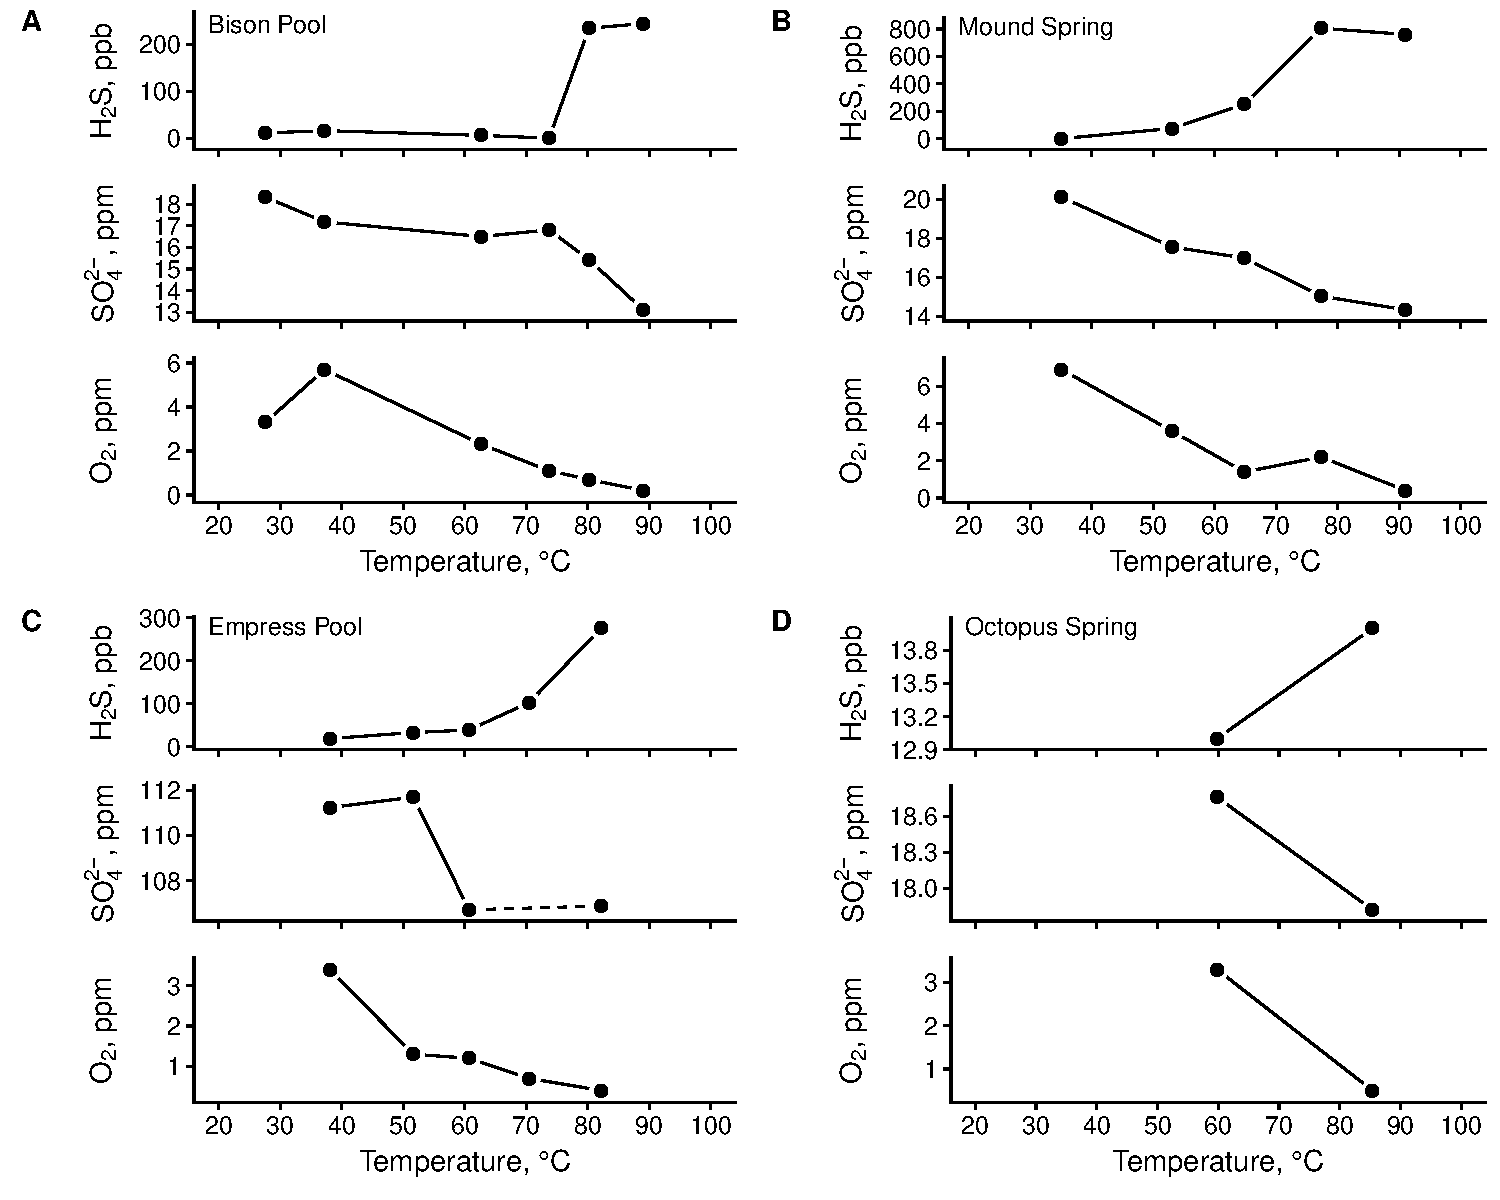
\includegraphics[width=1\linewidth]{figs_ch1/scatterplot_-_hot_spring_redox.pdf}
\caption[Concentrations of redox-sensitive aqueous chemical species in samples from Bison Pool, Mound Spring, Empress Pool, and Octopus Spring]{Concentrations of redox-sensitive aqueous chemical species in samples from Bison Pool (A), Mound Spring (B), Empress Pool (C) and Octopus Spring (D). Lines between points are meant to guide the eye between measurements only. A water sample could not be collected for sulfate at Empress Pool site EP2 during the 2012 field season, indicated here by a dashed line between sulfate measurements for sites EP1 and EP3.}
\label{fig:redox}
\end{figure}
\doublespace

% Capital letter 'numbering' assigned to subfigures with:
% \renewcommand{\thesubfigure}{\Alph{subfigure}}

\singlespace
\begin{figure}[h]
\centering
    \begin{subfigure}[b]{.3\linewidth}
        	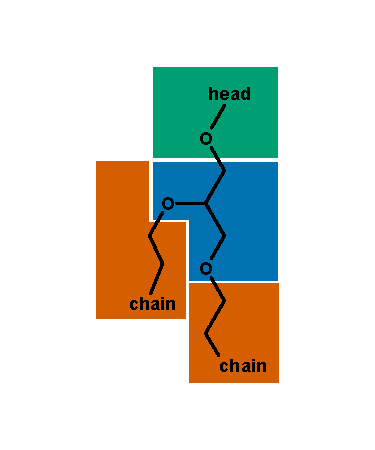
\includegraphics[width=1\linewidth]{figs_ch1/DEG}
        	\caption{DEG}
        \label{fig:DEG}
    \end{subfigure}
    \begin{subfigure}[b]{.3\linewidth}
    	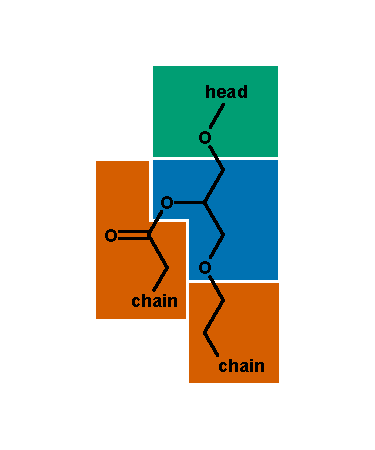
\includegraphics[width=1\linewidth]{figs_ch1/AEG}
    	\caption{AEG}
        \label{fig:AEG}
    \end{subfigure}
    \begin{subfigure}[b]{.3\linewidth}
        	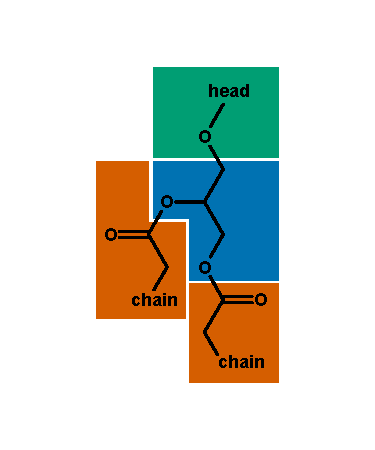
\includegraphics[width=\linewidth]{figs_ch1/DAG}
    	\caption{DAG}
        \label{fig:DAG}
    \end{subfigure}
    \begin{subfigure}[b]{.3\linewidth}
    	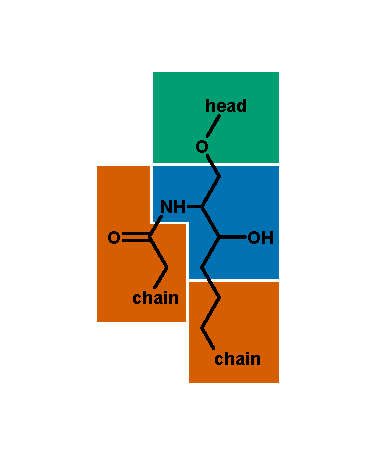
\includegraphics[width=\linewidth]{figs_ch1/CER}
    	\caption{CER}
        \label{fig:CER}
    \end{subfigure}
    \begin{subfigure}[b]{.3\linewidth}
    	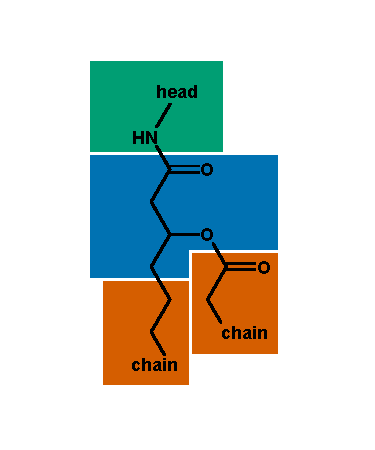
\includegraphics[width=\linewidth]{figs_ch1/FAHFAm}
    	\caption{FAHFAm}
        \label{fig:FAHFAm}
    \end{subfigure}
    \begin{subfigure}[b]{.3\linewidth}
        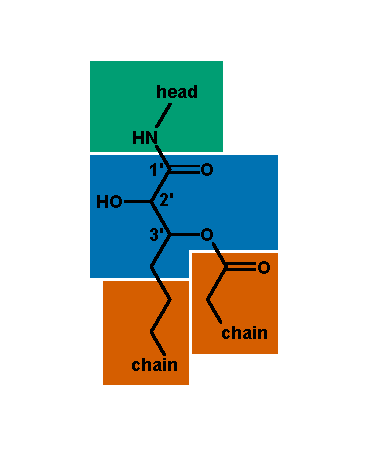
\includegraphics[width=\linewidth]{figs_ch1/FAHFAm-OH}
    	\caption{FAHFAm-OH*}
        \label{fig:FAHFAm-OH}
    \end{subfigure}
    \begin{subfigure}[b]{.6\linewidth}
        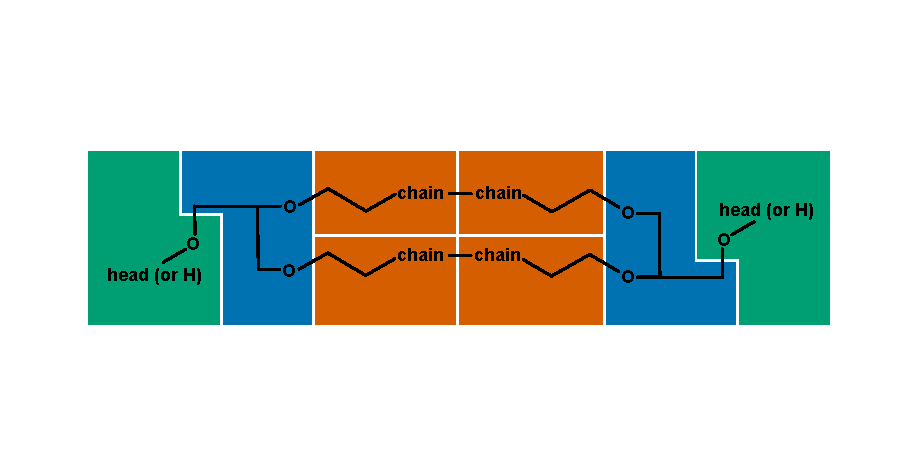
\includegraphics[width=\linewidth]{figs_ch1/GDGT}
    	\caption{GDGT}
        \label{fig:GDGT}
    \end{subfigure}
    \begin{subfigure}[b]{.3\linewidth}
    	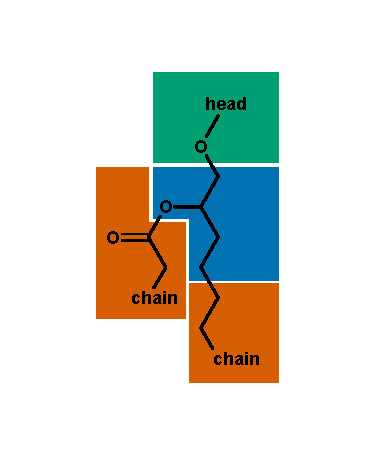
\includegraphics[width=\linewidth]{figs_ch1/alkanediol}
    	\caption{1,2-alkanediol}
        \label{fig:diol}
    \end{subfigure}
\end{figure}
\newpage
\begin{figure}[h]\ContinuedFloat

    \begin{subfigure}[b]{.3\linewidth}
    	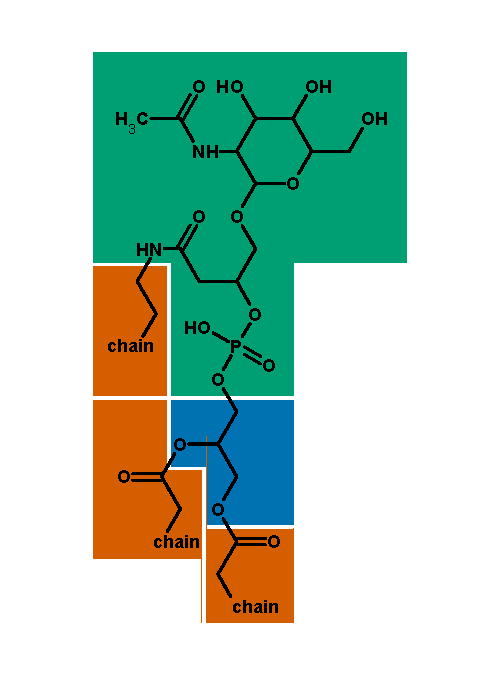
\includegraphics[width=\linewidth]{figs_ch1/NAcG-P-DAG}
    	\caption{NAcG-P-DAG}
        \label{fig:NAcG-P-DAG}
    \end{subfigure}
    \begin{subfigure}[b]{.3\linewidth}
    	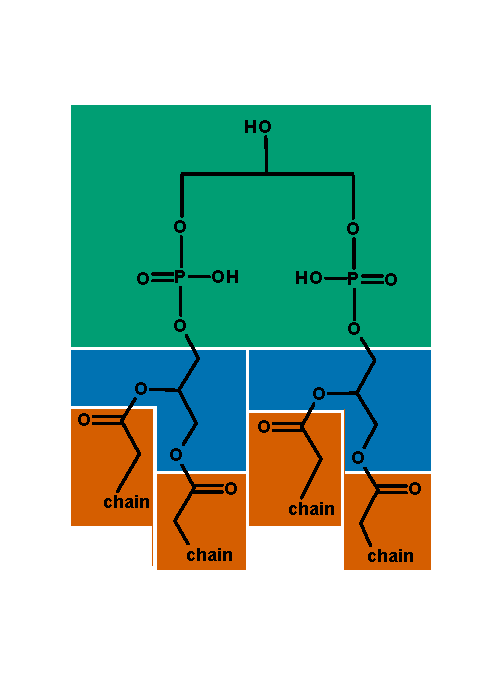
\includegraphics[width=\linewidth]{figs_ch1/DPG}
    	\caption{DPG}
        \label{fig:DPG}
    \end{subfigure}
    \begin{subfigure}[b]{.3\linewidth}
        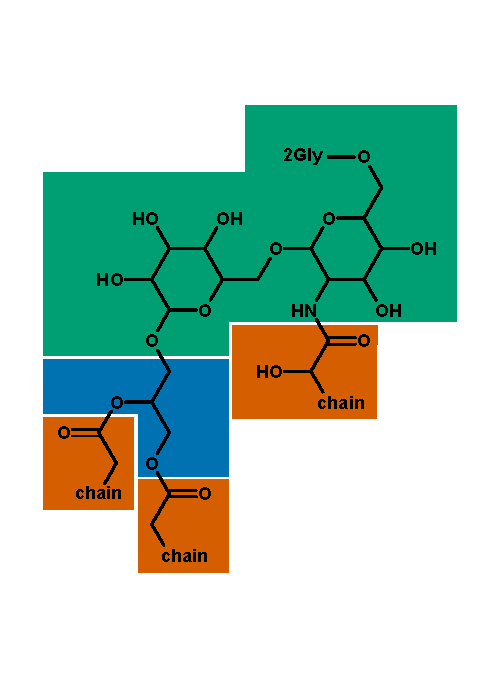
\includegraphics[width=\linewidth]{figs_ch1/2GNAcG-G-DAG}
    	\caption{2GNAcG-G-DAG**}
        \label{fig:2GNAcG-G-DAG}
    \end{subfigure}

    
\caption[Structural designations used for IPL headgroups, backbones, and alkyl chains]{Structural designations used for IPL headgroups, backbones, and alkyl chains for the sake of calculating abundance-weighted average properties and chemical formulas. Rules used to perform these designations are described in the text. Green boxes contain elemental abundances associated with headgroups, with only the headgroup-backbone connector group explicitly shown and the rest of the headgroup represented as `head'. Chemical formulae given in Table \ref{tab:IPL} represent elemental abundances of structures contained within the green box. Blue boxes contain `backbone' elemental abundances. Orange boxes designate elemental abundances belonging to alkyl chains. Only the chemical structure of the first two carbons of each alkyl chain are shown; with `chain' representing the rest. *In FAHFAm-OH, alkyl chain esterification may occur at either the 2' or 3' hydroxyl group \citep{diercks2015accumulation}. **NAcG-DAG in \cite{schubotz2013spatial}}
\label{fig:IPLdivision}
\end{figure}
\doublespace



\singlespace
\begin{figure}[h]
\centering
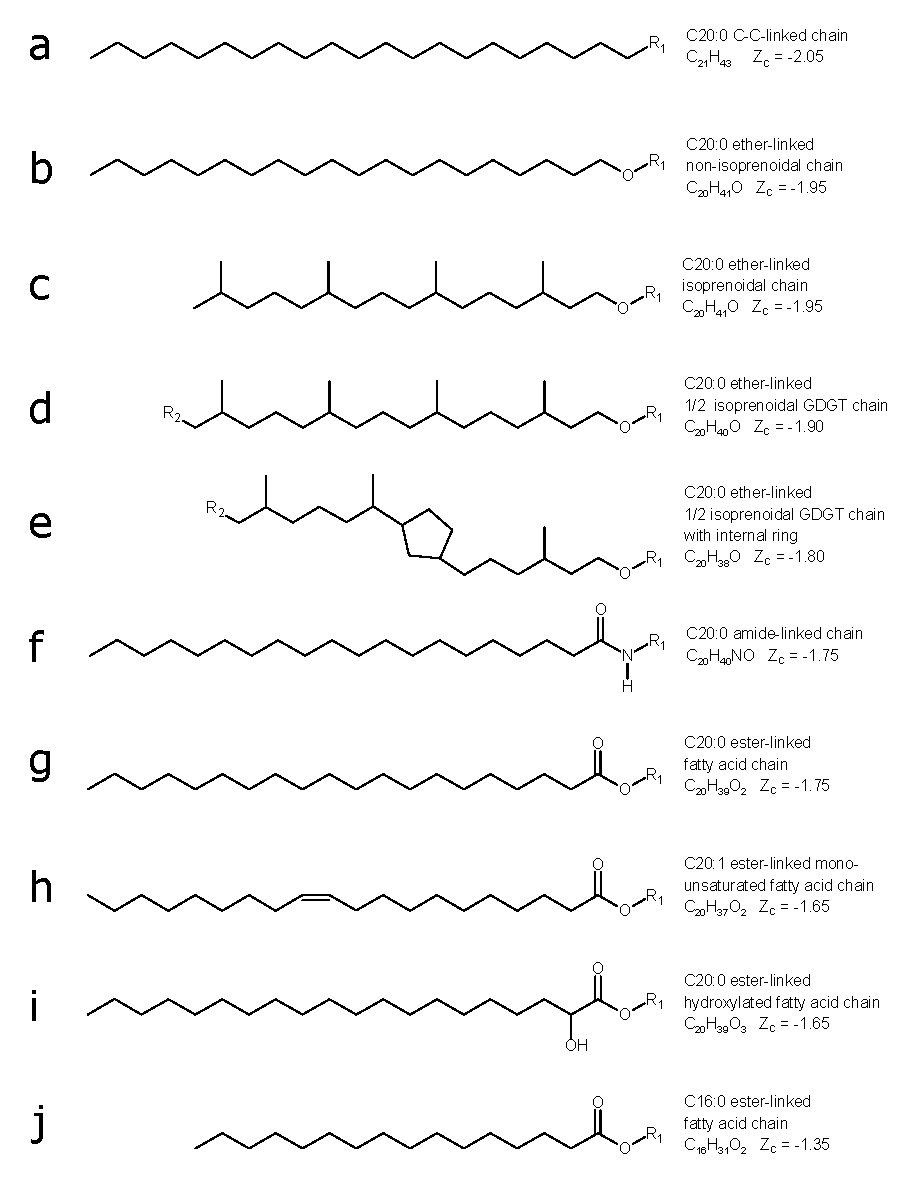
\includegraphics[width=.85\linewidth]{figs_ch1/chain_comparison}
\caption[Lipid alkyl chain modifications and backbone-chain linkage types organized by Z\textsubscript{C}]{Lipid alkyl chain modifications and backbone-chain linkage types organized by Z\textsubscript{C} from reduced (top) to oxidized (bottom). Example structures were chosen to permit comparison of Z\textsubscript{C} according to a single type of biochemical modification: chain-backbone linkage type as C-C, ether, amide, or ester (a, b, f, g); non-branching and branching chains (b, c); bilayer- and monolayer-forming isoprenoidal chains (c, d); GDGT chains without and with an internal ring (d, e); saturated and unsaturated chains (g, h); non-hydroxylated and hydroxylated chains (g, i); and chains with a greater and lesser number of aliphatic carbons (g, j). R\textsubscript{1} and R\textsubscript{2} represent a lipid backbone and the second half of a monolayer-forming GDGT chain, respectively.}
\label{fig:chain_comparison}
\end{figure}
\doublespace


\singlespace
\begin{figure}[h]
\centering
    \begin{subfigure}[b]{0.81\linewidth}
        	\includegraphics[width=1\linewidth]{"figs_ch1/scatterplot - weighted ZC of IPL components vs temp and logO2"}
    \end{subfigure}
    \begin{subfigure}[b]{0.18\linewidth}
        	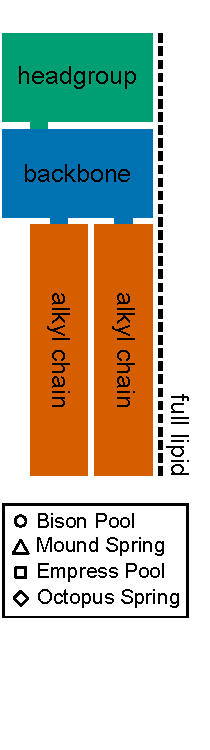
\includegraphics[width=1\linewidth]{figs_ch1/BasicLipidSchematic.pdf}
    \end{subfigure}
\caption[Abundance-weighted Z\textsubscript{C} of IPLs and their component parts]{Abundance-weighted Z\textsubscript{C} of headgroups (green), backbones (blue), alkyl chains (orange) and full (black) thermophile IPLs sampled along the outflow channels of four Yellowstone hot springs with respect to temperature (left) and log molality of dissolved O\textsubscript{2} (right). The observed value at each sample site are shown by points, while bars give the standard deviation of weighted Z\textsubscript{C} calculated over 999 bootstrap iterations, wherein underlying integrated HPLC-MS peak areas of individual IPLs were varied randomly by up to 30\% and analytical response factors assigned to each headgroup-backbone combination varied between 0.01$\times$ to 100$\times$ their original value. Lines of best fit indicate linear regression of all 999 bootstrap weighted Z\textsubscript{C}. Shaded areas represent 95\% prediction intervals for future bootstrap Z\textsubscript{C} results.}
\label{fig:weighted_ZC}
\end{figure}
\doublespace

\singlespace
\begin{figure}[h]
\centering
\includegraphics[width=1\linewidth]{"figs_ch1/boxplot - alkyl chain and full IPL ZC"}
\caption[Z\textsubscript{C} of IPLs and alkyl chains as a function of temperature]{Z\textsubscript{C} of IPLs (black/gray series) and their alkyl chains (orange series) as a function of temperature. Circles show weighted Z\textsubscript{C} of the full IPL or alkyl chains at each sample site. Rectangles show the interquartile range (IQR) of observed IPL and akyl chain Z\textsubscript{C}, with 25\% of observations lying above and below the black middle line, representing the median Z\textsubscript{C}, with whiskers encompassing observations up to 1.5 times the IQR beyond this range. Z\textsubscript{C} of IPLs that fall outside the range of the whiskers are not indicated. Linear regressions and 95\% confidence intervals are shown for weighted Z\textsubscript{C} (solid line with lighter confidence band) and for Z\textsubscript{C} of unweighted observations (dotted line with lighter confidence band).}
\label{fig:ZC}
\end{figure}
\doublespace


\singlespace
\begin{figure}[h]
\centering
\includegraphics[width=1\linewidth]{"figs_ch1/boxplot - headgroup ZC"}
\caption[Z\textsubscript{C} of IPL headgroups as a function of temperature]{Z\textsubscript{C} of IPL headgroups as a function of temperature. Circles show weighted Z\textsubscript{C} at each sample site. Rectangles show the interquartile range (IQR) of observed IPL headgroup Z\textsubscript{C}, with 25\% of observations lying above and below the black middle line, representing the median Z\textsubscript{C}, with whiskers encompassing observations up to 1.5 times the IQR beyond this range. Z\textsubscript{C} of IPL headgroups that fall outside the range of the whiskers are not indicated. Linear regressions and 95\% confidence intervals are shown for weighted Z\textsubscript{C} (solid line with lighter confidence band) and for Z\textsubscript{C} of unweighted observations (dotted line with lighter confidence band).}
\label{fig:ZC}
\end{figure}
\doublespace


\singlespace
\begin{figure}[h]
\centering
\includegraphics[width=.75\linewidth]{"figs_ch1/barplot - IPL chain linkage relative abundances"}
\caption[Relative abundance of backbone-alkyl chain linkage types]{Relative abundance of backbone-alkyl chain linkage types. Examples of C-C, ether, amide, and ester-linked alkyl chains are compared in Figure \ref{fig:chain_comparison}a, b, f, and g, respectively.}
\label{fig:IPL_linkage}
\end{figure}
\doublespace

\singlespace
\begin{figure}[h]
\centering
\includegraphics[width=1\linewidth]{"figs_ch1/boxplot - alkyl chain nC"}
\caption[Number of aliphatic carbons per IPL alkyl chain]{Number of aliphatic carbons per IPL alkyl chain. Dark points represent the weighted value, nC, while the box and whisker plots indicate distributions of individual IPL observations at each sample site, with the black horizontal bar representing the median.}
\label{fig:nC}
\end{figure}
\doublespace


\singlespace
\begin{figure}[h]
\centering
\includegraphics[width=1\linewidth]{"figs_ch1/boxplot - alkyl chain nUnsat"}
\caption[Number of unsaturations per IPL alkyl chain]{Number of unsaturations per IPL alkyl chain. Dark points represent the weighted value, nUnsat, while the box and whisker plots indicate distributions of individual IPL observations at each sample site, with the black horizontal bar representing the median.}
\label{fig:nUnsat}
\end{figure}
\doublespace


\singlespace
\begin{figure}[h]
\centering
\includegraphics[width=1\linewidth]{"figs_ch1/boxplot - alkyl chain nRings"}
\caption[Number of internal rings per GDGT]{Number of internal rings per GDGT. Dark points represent the weighted value, while the box and whisker plots indicate distributions of individual IPL observations at each sample site, with the black horizontal bar representing the median.}
\label{fig:nRings}
\end{figure}
\doublespace